\section{Know your tools}\label{sec:tools}
%
Jolla chose the Qt framework to be part of their technology stack.
``Qt is a cross-platform application and UI framework for developers using C++ or QML, a CSS \& JavaScript like language. Qt Creator is the supporting Qt IDE.
Qt, Qt Quick and the supporting tools are developed as an open source project governed by an inclusive meritocratic model. Qt can be used under open source (LGPL v2.1) or commercial terms.''\cite{qt01}

``Qt - code once, deploy everywhere'', that's the mantra of the Qt framework. If you have developed for more than one platform in the past, you know that this sounds like heaven. Maintaining different source code and technologies for each and every platform is a tedious task that can eat up all your developer resources. As if software development is not difficult enough if you stay on one platform\footnote{In my eyes software development is an art of craftsmanship and can not be done by Mr. Average and thus is a more or less complicated thing to do.}.

So there were good reasons to choose Qt as framework, no doubt about that. As of now you can develop for Android, iOS, BlackBerry and of course SailfishOS. If you look into the documentation and examples of all these platforms, you will find that those examples assume, that you are developing for this platform only. Quite stupid, if you use the Qt framework. Understandable if you think about the effort that would be necessary to build a documentation that incorporates all other possible platforms. For some time now I was wondering how I should organize my code in such a way, that allows me to develop for more than one target platform at a time. It's not just compiling for another platform! Each platform has a unique UI that behaves in an own different way, e.g. SailfishOS is gesture based, other ones are touch based.
In the long run you will create an UI for each of those targets. Period. Patterns like MVC\cite{wiki01} will come to mind, using separate business logic, yada yada.

To cut a long story short, why am I writing about this stuff, this section is supposed to be about tools? When you prepare a software project for the use for more than one target platform, you will start organizing stuff differently. Maybe you use folders that have the name of the targets to differentiate stuff that's platform dependent. Maybe you even create a business logic that is really unique and capsulated in such clever way that it can be reused and does not know anything about the outside world. Such a business logic or model can be driven from tests, command line tools, web or different native UIs. Would be nice to have it in a separate folder or even subproject. If you start to move and/or rename things, your tools will break. Intentionally.

By examining those fractures you can learn a lot about your tools that otherwise work so silently in the background. So go on and break your tools!\footnote{Ok, not so short :-)}

Here is what I've learned so far.
%
\subsection{Technology stack}
%
\begin{figure}[H]
  \centering
  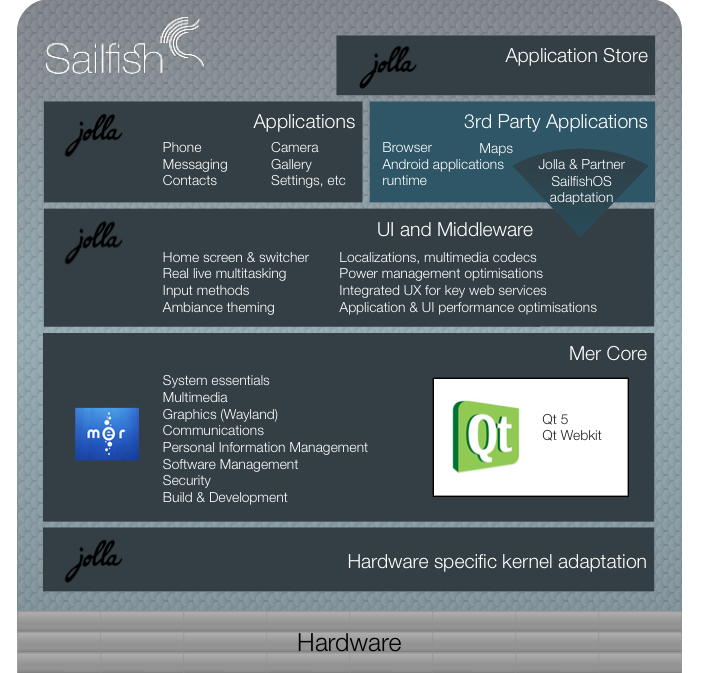
\includegraphics[scale=0.8]{../media/gfx/Sailfish/Sailfish_Architecture.png} 
  \caption{Sailfish architecture, taken from\\https://sailfishos.org/images/Sailfish\_Architecture.png.}
  \label{fig:SailfishArchitecture}
\end{figure}
%
\subsection{QtCreator integrated development environment (IDE)}\label{subset:QtCreator}
%
``QtCreator is a cross platform integrated development environment (IDE) tailored to the needs of Qt developers. It has been extended to add support for Sailfish UI application development using Sailfish Silica components. It provides a sophisticated code editor with version control, project and build management system integration.''\cite{sailfishos3}.

Reusing an existing open source IDE is a smart move from Jolla. Why should they waste resources on developing something that has already done by others? Or why should they burn up their staff for all those development solutions out there? Be it Visual Studio, Eclipse, Emacs or even Vi. If you really dive in the tools, you can also use those but I doubt that Jolla will provide you with support if something does not work. Working with QtCreator is also quite natural in the Qt universe albeit being a fast IDE. So have a look in the preferences\footnote{On Windows and Linux they should be found in Extras/Options.}.
\begin{figure}[H]
  \centering
  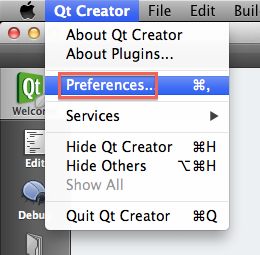
\includegraphics[scale=0.7]{../media/gfx/QtCreator/QtCreatorPreferences.png} 
  \caption{Open the QtCreator preferences.}
  \label{fig:creatorpref}
\end{figure}
%
I will not walk through every setting of QtCreator, \cite{qt02} is a better place to start for basic questions.
Also I will not use the order of tabs in the preferences, but try to follow the sequence in which those tools touch your source code.
%
%
\subsubsection{kits}\label{subsubsec:kits}
%
But before we do that, we must talk about \textit{kits}. A kit is kind of an umbrella setting, which combines the information of the following bits and pieces, like \verb,qmake,, \verb,compiler,, and \verb,device type,. This is the information hub that QtCreator uses to pull all information together and initiate its actions when you build or start your application.
%
\begin{figure}[H]
  \centering
  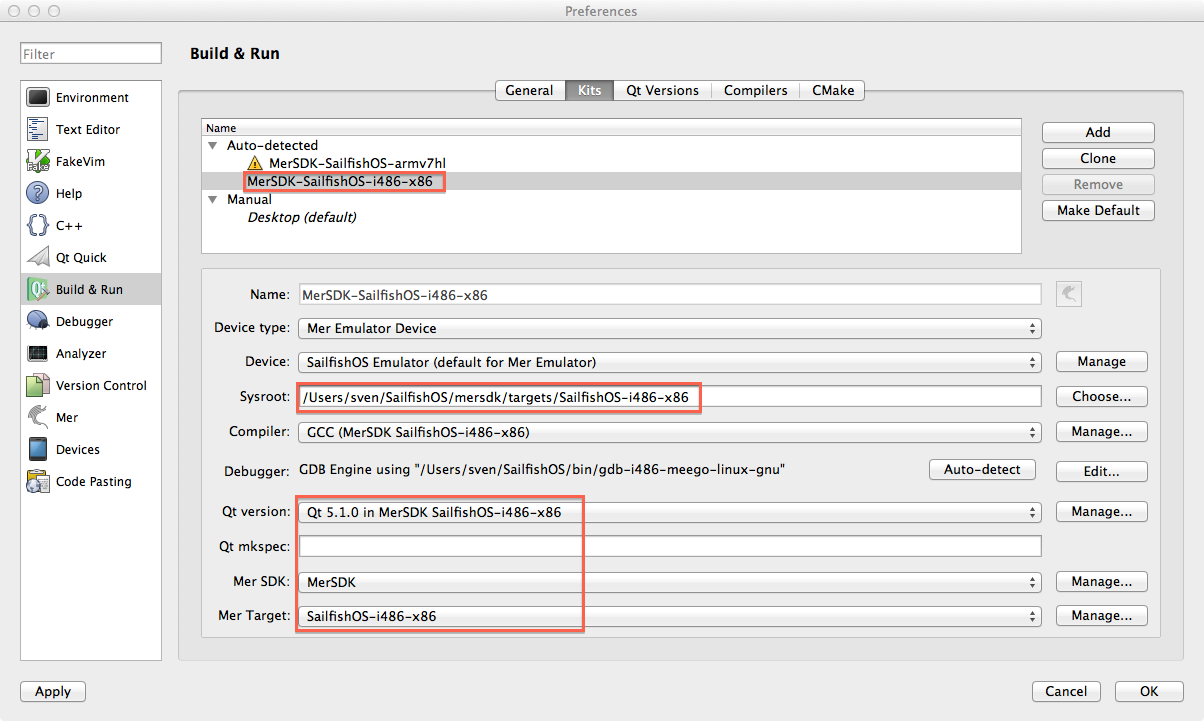
\includegraphics[scale=0.35]{../media/gfx/QtCreator/kits486.png} 
  \caption{Preferences, kits tab.}
  \label{fig:creatorkits}
\end{figure}
%
So far there are 2 kits defined:
\begin{itemize}
\item MerSDK-SailfishOS-armv7hl \\
		\emph{this kit is marked with a warning sign in the Alpha2 SDK, there is no device assigned yet.\\
		The Alph3 SDK brings device support but it's not configured yet.}
\item MerSDK-SailfishOS-i486-x86
\end{itemize}
%
Should you have a kit named \verb,Desktop,, it's of no use inside the QtCreator that comes with the SailfishOS SDK, try not to build your app with this kit!
%
\subsubsection{qmake}\label{subsubsec:qmake}
%
\begin{figure}[H]
  \centering
  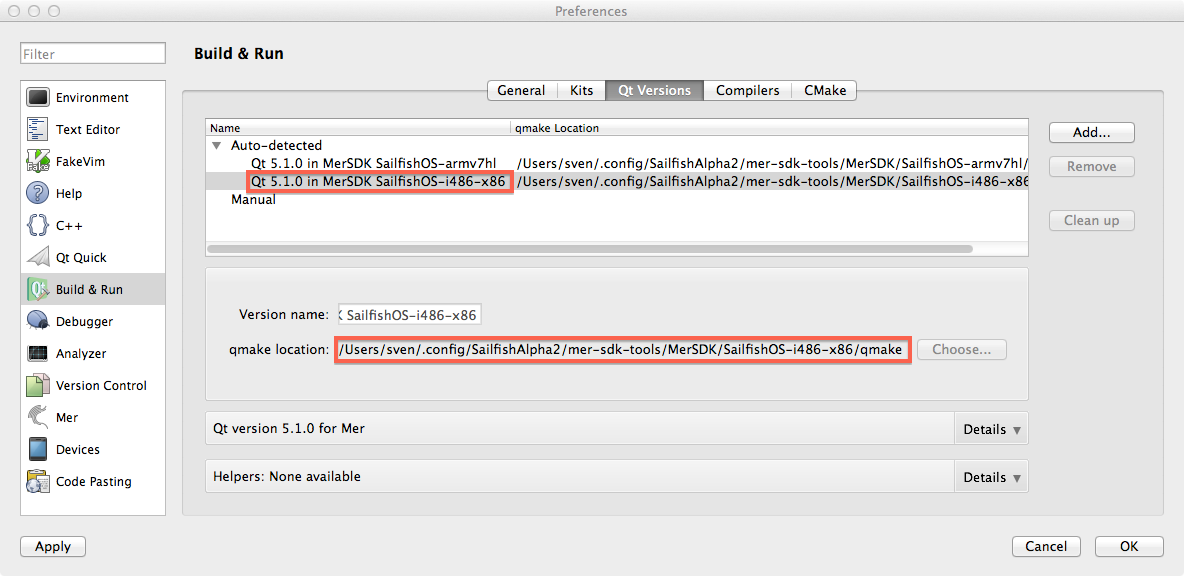
\includegraphics[scale=0.35]{../media/gfx/QtCreator/QtCreatorQtVersions.png} 
  \caption{Preferences, QtVersions tab.}
  \label{fig:qmake486pref}
\end{figure}
%
``qmake is a tool that helps simplify the build process for development project across different platforms. qmake automates the generation of Makefiles so that only a few lines of information are needed to create each Makefile. qmake can be used for any software project, whether it is written in Qt or not.
qmake generates a Makefile based on the information in a project file. Project files are created by the developer, and are usually simple, but more sophisticated project files can be created for complex projects. qmake contains additional features to support development with Qt, automatically including build rules for moc and uic. qmake can also generate projects for Microsoft Visual studio without requiring the developer to change the project file.''\cite{qt03}
%
\begin{figure}[H]
  \centering
  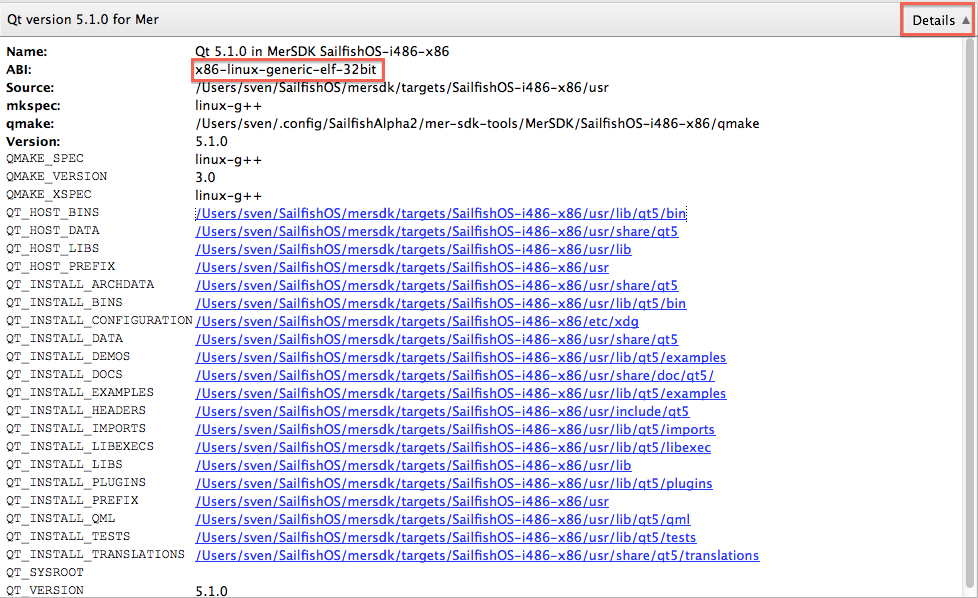
\includegraphics[scale=0.45]{../media/gfx/QtCreator/qmakedetails.png} 
  \caption{Preferences, QtVersions tab., qmake details}
  \label{fig:qmakedetailspref}
\end{figure}
%
UIC is a tool that creates C++ classes from XML information generated with the UI designer inside QtCreator. This designer is for Qt widgets which should not be used with SailfishOS and is not further explained in this document.

MOC is the Meta-Object Compiler which ``reads a C++ header file. If it finds one or more class declarations that contain the \verb,Q_OBJECT, macro, it produces a C++ source file containing the meta-object code for those classes.''\cite{qt04}. If you use \verb,qmake, to produce your Makefile, you don't have to worry about it, the rules are created automatically.
%
\begin{figure}[H]
  \centering
  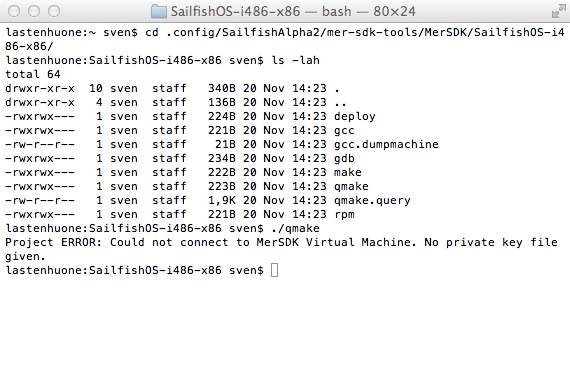
\includegraphics[scale=0.6]{../media/gfx/bash/qmake486.png} 
  \caption{Running qmake from command line.}
  \label{fig:qmake486commandline}
\end{figure}
%
If you run qmake manually, you will find out that it tries to connect to the \textit{Mer build engine for cross compilation}. The error also appears if the virtual machine is up and running. In the Projects settings you can see how \verb,qmake, is invoked if started by QtCreator.
%
\begin{figure}[H]
  \centering
  
\includegraphics[scale=0.8]{../media/gfx/QtCreator/projects.png} 
  \caption{Project settings.}
  \label{fig:qmakeprojectsettings}
\end{figure}
%
%
\begin{figure}[H]
  \centering
  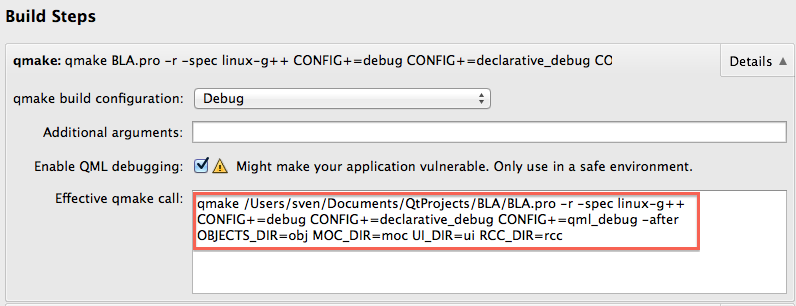
\includegraphics[scale=0.5]{../media/gfx/QtCreator/buildstepsqmake.png} 
  \caption{Build steps for qmake.}
  \label{fig:qmakebuildsteps}
\end{figure}
%
Using those parameters via command line does not work, too.
\begin{figure}[H]
  \centering
  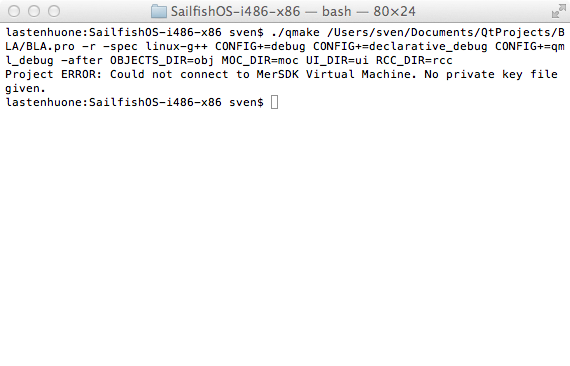
\includegraphics[scale=0.6]{../media/gfx/bash/qmakewithparam.png} 
  \caption{Running qmake from command line with parameters from build steps.}
  \label{fig:qmake486buildstepsparamcommandline}
\end{figure}
%
If \verb,qmake, is invoked by the QtCreator it works just fine.
\begin{figure}[H]
  \centering
  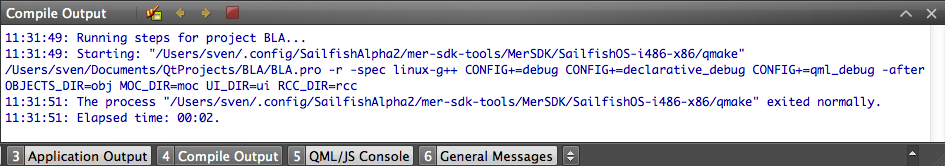
\includegraphics[scale=0.5]{../media/gfx/QtCreator/qmakerunfromqtcreator.png} 
  \caption{Running qmake from QtCreator (Build menu).}
  \label{fig:qmake486runfromqtcreator}
\end{figure}
%
As a result you will find a \verb,Makefile, in your project directory.
\begin{figure}[H]
  \centering
  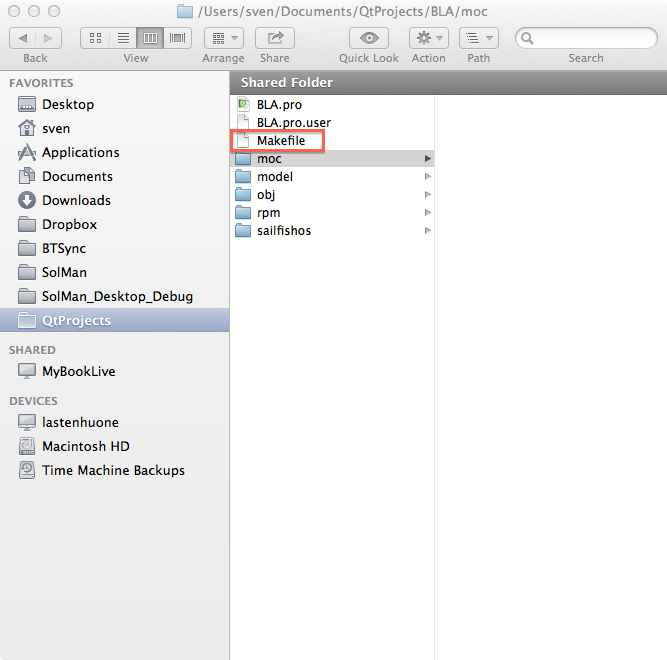
\includegraphics[scale=0.5]{../media/gfx/QtCreator/qmakeresult.png} 
  \caption{Result of running qmake from QtCreator (Build menu).}
  \label{fig:qmake486result}
\end{figure}
%
Here is the snippet about the MOC.
%
\begin{lstlisting}[language=make]
####### Sub-libraries

distclean: clean
	-$(DEL_FILE) $(TARGET) 
	-$(DEL_FILE) Makefile


mocclean: compiler_moc_header_clean compiler_moc_source_clean

mocables: compiler_moc_header_make_all compiler_moc_source_make_all

check: first

compiler_rcc_make_all:
compiler_rcc_clean:
compiler_wayland-server-header_make_all:
compiler_wayland-server-header_clean:
compiler_wayland-client-header_make_all:
compiler_wayland-client-header_clean:
compiler_qtwayland-client-header_make_all:
compiler_qtwayland-client-header_clean:
compiler_qtwayland-server-header_make_all:
compiler_qtwayland-server-header_clean:
compiler_moc_header_make_all: moc/moc_qbusinesslogic.cpp
compiler_moc_header_clean:
	-$(DEL_FILE) moc/moc_qbusinesslogic.cpp
moc/moc_qbusinesslogic.cpp: /usr/include/qt5/QtCore/QObject \
		/usr/include/qt5/QtCore/qobject.h \
		/usr/include/qt5/QtCore/qobjectdefs.h \
		/usr/include/qt5/QtCore/qnamespace.h \
		/usr/include/qt5/QtCore/qglobal.h \
		/usr/include/qt5/QtCore/qconfig.h \
		/usr/include/qt5/QtCore/qfeatures.h \
		/usr/include/qt5/QtCore/qsystemdetection.h \
		/usr/include/qt5/QtCore/qcompilerdetection.h \
		/usr/include/qt5/QtCore/qprocessordetection.h \
		/usr/include/qt5/QtCore/qglobalstatic.h \
		/usr/include/qt5/QtCore/qatomic.h \
		/usr/include/qt5/QtCore/qbasicatomic.h \
		/usr/include/qt5/QtCore/qatomic_bootstrap.h \
		/usr/include/qt5/QtCore/qgenericatomic.h \
		/usr/include/qt5/QtCore/qatomic_msvc.h \
		/usr/include/qt5/QtCore/qatomic_integrity.h \
		/usr/include/qt5/QtCore/qoldbasicatomic.h \
		/usr/include/qt5/QtCore/qatomic_vxworks.h \
		/usr/include/qt5/QtCore/qatomic_power.h \
		/usr/include/qt5/QtCore/qatomic_alpha.h \
		/usr/include/qt5/QtCore/qatomic_armv7.h \
		/usr/include/qt5/QtCore/qatomic_armv6.h \
		/usr/include/qt5/QtCore/qatomic_armv5.h \
		/usr/include/qt5/QtCore/qatomic_bfin.h \
		/usr/include/qt5/QtCore/qatomic_ia64.h \
		/usr/include/qt5/QtCore/qatomic_mips.h \
		/usr/include/qt5/QtCore/qatomic_s390.h \
		/usr/include/qt5/QtCore/qatomic_sh4a.h \
		/usr/include/qt5/QtCore/qatomic_sparc.h \
		/usr/include/qt5/QtCore/qatomic_x86.h \
		/usr/include/qt5/QtCore/qatomic_cxx11.h \
		/usr/include/qt5/QtCore/qatomic_gcc.h \
		/usr/include/qt5/QtCore/qatomic_unix.h \
		/usr/include/qt5/QtCore/qmutex.h \
		/usr/include/qt5/QtCore/qlogging.h \
		/usr/include/qt5/QtCore/qflags.h \
		/usr/include/qt5/QtCore/qtypeinfo.h \
		/usr/include/qt5/QtCore/qtypetraits.h \
		/usr/include/qt5/QtCore/qsysinfo.h \
		/usr/include/qt5/QtCore/qobjectdefs_impl.h \
		/usr/include/qt5/QtCore/qstring.h \
		/usr/include/qt5/QtCore/qchar.h \
		/usr/include/qt5/QtCore/qbytearray.h \
		/usr/include/qt5/QtCore/qrefcount.h \
		/usr/include/qt5/QtCore/qarraydata.h \
		/usr/include/qt5/QtCore/qstringbuilder.h \
		/usr/include/qt5/QtCore/qlist.h \
		/usr/include/qt5/QtCore/qalgorithms.h \
		/usr/include/qt5/QtCore/qiterator.h \
		/usr/include/qt5/QtCore/qcoreevent.h \
		/usr/include/qt5/QtCore/qscopedpointer.h \
		/usr/include/qt5/QtCore/qmetatype.h \
		/usr/include/qt5/QtCore/qvarlengtharray.h \
		/usr/include/qt5/QtCore/qcontainerfwd.h \
		/usr/include/qt5/QtCore/qisenum.h \
		/usr/include/qt5/QtCore/qobject_impl.h \
		model/qt/qbusinesslogic.h
	/usr/lib/qt5/bin/moc $(DEFINES) $(INCPATH) -I/usr/lib/gcc/i486-meego-linux/4.6.4/../../../../include/c++/4.6.4 -I/usr/lib/gcc/i486-meego-linux/4.6.4/../../../../include/c++/4.6.4/i486-meego-linux -I/usr/lib/gcc/i486-meego-linux/4.6.4/../../../../include/c++/4.6.4/backward -I/usr/lib/gcc/i486-meego-linux/4.6.4/include -I/usr/local/include -I/usr/include model/qt/qbusinesslogic.h -o moc/moc_qbusinesslogic.cpp
\end{lstlisting}
%
The \verb,qmake, from the SailfishOS SDK is just a simple bash script, that invokes \verb,merssh,.
%
\begin{lstlisting}[language=bash]
#!/bin/bash
exec "/Users/sven/SailfishOS/bin/Qt Creator.app/Contents/MacOS/../Resources/merssh" -sdktoolsdir "/Users/sven/.config/SailfishAlpha3/mer-sdk-tools/MerSDK" -commandtype mb2 -mertarget SailfishOS-i486-x86 qmake $@oluhuone:SailfishOS-i486-x86
\end{lstlisting}
%
So that's the trick: \verb,$@, is replaced with the \verb,qmake, call parameters, \verb,oluhuone, is just the name of one of my computers.
%
%
\subsubsection{.pro file}
%
Project files contain all the information required by \nameref{subsubsec:qmake} to build your application, library, or plugin. Generally, you use a series of declarations to specify the resources in the project, but support for simple programming constructs enables you to describe different build processes for different platforms and environments[QtCreator help].

If you select the help mode of QtCreator and switch to \emph{Index}, you can search amongst other things for \verb,qmake, and have a look at the \verb,qmake Variable Reference,.
%
\begin{figure}[H]
  \centering
  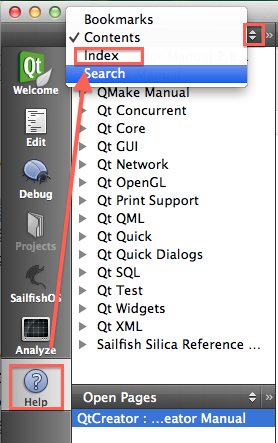
\includegraphics[scale=0.7]{../media/gfx/QtCreator/HelpSelectIndex.png} 
  \caption{QtCreator, Help, Index.}
  \label{fig:HelpSelectIndex}
\end{figure}
%
The fundamental behavior of qmake is influenced by variable declarations that define the build process of each project. Some of these declare resources, such as headers and source files, that are common to each platform. Others are used to customize the behavior of compilers and linkers on specific platforms[QtCreator help].
%
\begin{figure}[H]
  \centering
  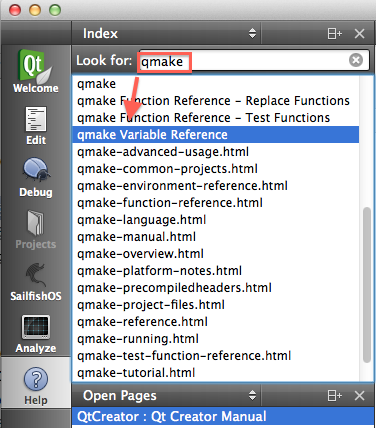
\includegraphics[scale=0.7]{../media/gfx/QtCreator/HelpSearchQmake.png} 
  \caption{QtCreator, search for qmake.}
  \label{fig:HelpSearchQmake}
\end{figure}
%
The \verb,.pro, file from a new created SailfishOS application looks like
%
\begin{lstlisting}[language=tex]
# The name of your app.
# NOTICE: name defined in TARGET has a corresponding QML filename.
#         If name defined in TARGET is changed, following needs to be
#         done to match new name:
#         - corresponding QML filename must be changed
#         - desktop icon filename must be changed
#         - desktop filename must be changed
#         - icon definition filename in desktop file must be changed
TARGET = NAME_OF_THEAPP

CONFIG += sailfishapp

SOURCES += src/NAME_OF_THEAPP.cpp

OTHER_FILES += qml/NAME_OF_THEAPP.qml \
    qml/cover/CoverPage.qml \
    qml/pages/FirstPage.qml \
    qml/pages/SecondPage.qml \
    rpm/NAME_OF_THEAPP.spec \
    rpm/NAME_OF_THEAPP.yaml \
    NAME_OF_THEAPP.desktop
\end{lstlisting}
%
The target is the name of the compiled binary.
%
\begin{lstlisting}[language=tex]
TARGET = NAME_OF_THEAPP
\end{lstlisting}
%
All SailfishOS silica application share some common settings, those are imported with the \verb,sailfishapp.prf, Qt feature file.
%
\begin{lstlisting}[language=tex]
CONFIG += sailfishapp
\end{lstlisting}
%
Your C++ implementation files are SOURCES\footnote{The corresponding header files are HEADERS.}.
%
\begin{lstlisting}[language=tex]
SOURCES += src/NAME_OF_THEAPP.cpp
\end{lstlisting}
%
All kind of resource files are the \verb,OTHER_FILES,.
%
\begin{lstlisting}[language=tex]
OTHER_FILES += qml/NAME_OF_THEAPP.qml \
    qml/cover/CoverPage.qml \
    qml/pages/FirstPage.qml \
    qml/pages/SecondPage.qml \
    rpm/NAME_OF_THEAPP.spec \
    rpm/NAME_OF_THEAPP.yaml \
    NAME_OF_THEAPP.desktop
\end{lstlisting}
%
More directives can be found in the help system.
%
%
\subsubsection{.prf file}
%
You may ask yourself what the \verb,CONFIG += sailfishapp, line does? It tells \verb,qmake, to include the content of the \verb,sailfishapp.prf, file while it processes the \verb,.pro, file of your application. Those files are called Qt feature files and work more or less like \verb,.pro, files. Their purpose is to share common configuration between different projects.

Have a look into the
%
\begin{lstlisting}[language=tex]
~/SailfishOS/mersdk/targets/SailfishOS-i486-x86/usr/share/qt5/mkspecs/features/
\end{lstlisting}
%
folder, there are some more\footnote{Those are actually copies to satisfy QtCreator. During compilation the same files stored on the Mer SDK virtual machine are used. Details can be found on \cite{sailfishos6}.}.
%
\begin{lstlisting}[language=tex]
#
# sailfishapp.prf: Qt Feature file for libsailfishapp
# Usage: CONFIG += sailfishapp
#
# Copyright (c) 2013 Jolla Ltd.
# Contact: Thomas Perl <thomas.perl@jollamobile.com>
# All rights reserved.
#
# This file is part of libsailfishapp
#
# You may use this file under the terms of BSD license as follows:
#
# Redistribution and use in source and binary forms, with or without
# modification, are permitted provided that the following conditions are met:
#     * Redistributions of source code must retain the above copyright
#       notice, this list of conditions and the following disclaimer.
#     * Redistributions in binary form must reproduce the above copyright
#       notice, this list of conditions and the following disclaimer in the
#       documentation and/or other materials provided with the distribution.
#     * Neither the name of the Jolla Ltd nor the
#       names of its contributors may be used to endorse or promote products
#       derived from this software without specific prior written permission.
#
# THIS SOFTWARE IS PROVIDED BY THE COPYRIGHT HOLDERS AND CONTRIBUTORS "AS IS" AND
# ANY EXPRESS OR IMPLIED WARRANTIES, INCLUDING, BUT NOT LIMITED TO, THE IMPLIED
# WARRANTIES OF MERCHANTABILITY AND FITNESS FOR A PARTICULAR PURPOSE ARE
# DISCLAIMED. IN NO EVENT SHALL THE COPYRIGHT HOLDERS OR CONTRIBUTORS BE LIABLE FOR
# ANY DIRECT, INDIRECT, INCIDENTAL, SPECIAL, EXEMPLARY, OR CONSEQUENTIAL DAMAGES
# (INCLUDING, BUT NOT LIMITED TO, PROCUREMENT OF SUBSTITUTE GOODS OR SERVICES;
# LOSS OF USE, DATA, OR PROFITS; OR BUSINESS INTERRUPTION) HOWEVER CAUSED AND
# ON ANY THEORY OF LIABILITY, WHETHER IN CONTRACT, STRICT LIABILITY, OR TORT
# (INCLUDING NEGLIGENCE OR OTHERWISE) ARISING IN ANY WAY OUT OF THE USE OF THIS
# SOFTWARE, EVEN IF ADVISED OF THE POSSIBILITY OF SUCH DAMAGE.
#

QT += quick qml

target.path = /usr/bin

qml.files = qml
qml.path = /usr/share/$${TARGET}

desktop.files = $${TARGET}.desktop
desktop.path = /usr/share/applications

icon.files = $${TARGET}.png
icon.path = /usr/share/icons/hicolor/86x86/apps

INSTALLS += target qml desktop icon

CONFIG += link_pkgconfig
PKGCONFIG += sailfishapp
INCLUDEPATH += /usr/include/sailfishapp

OTHER_FILES += $$files(rpm/*)
\end{lstlisting}
%
First of all two Qt modules are added to the project.
%
\begin{lstlisting}[language=tex]
QT += quick qml
\end{lstlisting}
%
Your target binary is copied to \verb,/usr/bin, when \verb,make, is called\footnote{Not really, this would happen if the program would be compiled and deployed on your development machine. See at the end of this section.}.
%
\begin{lstlisting}[language=tex]
target.path = /usr/bin
\end{lstlisting}
%
\verb,TARGET, is a special name in a Qt project configuration file. Other group of files can be named freely as long as they don't collide with qmake variable names. All files from the folder \emph{qml} will be installed in the directory\\ \verb,/usr/share/NAME_OF_THEAPP, \\The \verb,$${TARGET}, directive resolves to the content of the variable \verb,TARGET, and that's \verb,NAME_OF_THEAPP, in our case here.
%
\begin{lstlisting}[language=tex]
qml.files = qml
qml.path = /usr/share/$${TARGET}
\end{lstlisting}
%
The file \verb,NAME_OF_THEAPP.desktop, will be installed in the folder\\ \verb,/usr/share/applications,.
%
\begin{lstlisting}[language=tex]
desktop.files = $${TARGET}.desktop
desktop.path = /usr/share/applications
\end{lstlisting}
%
Your icon file \verb,NAME_OF_THEAPP.png, will be installed in\\ \verb,/usr/share/icons/hicolor/86x86/apps,.
%
\begin{lstlisting}[language=tex]
icon.files = $${TARGET}.png
icon.path = /usr/share/icons/hicolor/86x86/apps
\end{lstlisting}
%
If you run \verb,qmake, it will build a \verb,Makefile, which contains the rules to install four sets of files. First the target install set  which is built-in Qt projects.
%
\begin{lstlisting}[language=tex]
INSTALLS += target qml desktop icon
\end{lstlisting}
%
Then there are the remaining three as above self defined install sets \verb,qmk,, \verb,dektop, and \verb,icon,. When you \verb,make, your application the install sets will be processed in the given order.

This tells \verb,qmake, to make use of an external library that is supported by \nameref{subsubsec:pkgconfig}. The name of the external library is \verb,sailfishapp,.
%
\begin{lstlisting}[language=tex]
CONFIG += link_pkgconfig
PKGCONFIG += sailfishapp
\end{lstlisting}
%
When you compile your program the \verb,INCLUDEPATH, defines where \verb,#include,d header files are looked up.
%
\begin{lstlisting}[language=tex]
INCLUDEPATH += /usr/include/sailfishapp
\end{lstlisting}
%
All paths that are referenced in the \verb,.prf, file don't make sense on your development machine or on the Mer SDK virtual machine. They will be tweaked during building time. You can watch the command in the output tab of QtCreator, the call is actually\\
\verb,make install INSTALL_ROOT=/home/deploy/installroot,\\
So every path given in the \verb,.prf, file is relative to
\verb,/home/deploy/installroot, on the Mer SDK virtual machine. The files stay there after you have built the application and are the source for either \emph{Binary Copy Deployment} or \emph{RPM Deployment}.
%
%
\subsubsection{merssh}\label{subsubsec:merssh}
%
Looking with \verb,top, showed a process called \verb,merssh, when \verb,qmake, was started via QtCreator. Interesting, what's that?
%
\begin{figure}[H]
  \centering
  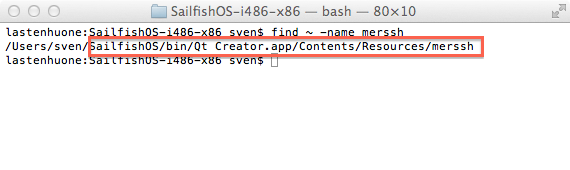
\includegraphics[scale=0.6]{../media/gfx/bash/merssh.png} 
  \caption{What is merssh?.}
  \label{fig:merssh}
\end{figure}
%
So it is part of the QtCreator that is shipped with the SailfishOS SDK.
%
\begin{figure}[H]
  \centering
  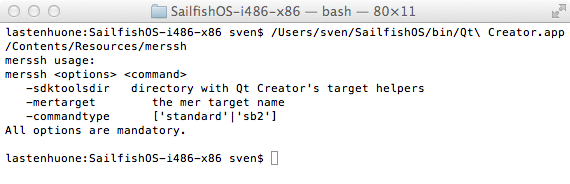
\includegraphics[scale=0.6]{../media/gfx/bash/mersshinvoked.png} 
  \caption{merssh invoked, what's it?.}
  \label{fig:mersshinvoked}
\end{figure}
%
All the programs called by QtCreator during the build and run process are more or less just proxy scripts\footnote{OSX and Linux come with bash scripts, Windows comes with?} that call \verb,merssh,, which in turn calls something on the \nameref{subsec:MerSDK}, see page \pageref{subsec:MerSDK}.

More than that, it calls \verb,sb2, which is short for Scratchbox2, have a look at section \nameref{subsec:scratchbox2} on page \pageref{subsec:scratchbox2}, there are more details. For now let's just assume that ``Scratchbox 2 is a cross-compilation engine, it can be used to create a highly flexible SDK.''\cite{sb2}.
%
\begin{figure}[H]
  \centering
  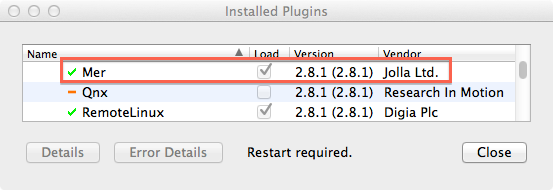
\includegraphics[scale=0.5]{../media/gfx/QtCreator/merplugin.png} 
  \caption{Mer plugin, maybe that's the source of merssh?.}
  \label{fig:merplugin}
\end{figure}
%
I've grepped the command line for the \verb,merssh,
\begin{lstlisting}[language=bash]
$ ps -ef|grep "merssh"
\end{lstlisting}
%
And the result is:
\begin{lstlisting}[language=bash]
/Users/sven/SailfishOS/bin/Qt Creator.app/Contents/MacOS/../Resources/merssh -sdktoolsdir /Users/sven/.config/SailfishAlpha3/mer-sdk-tools/MerSDK -commandtype mb2 -mertarget SailfishOS-i486-x86 qmake /Users/sven/QtProjects/TestSailfishOS/TestSailfishOS.pro -r -spec linux-g++ CONFIG+=debug CONFIG+=declarative_debug CONFIG+=qml_debug -after OBJECTS_DIR=obj MOC_DIR=moc UI_DIR=ui RCC_DIR=rcc
\end{lstlisting}
%
The picture is getting clearer now. QtCreator starts the SDK version of \verb,qmake, which call \verb,merssh, with all parameters needed to call \verb,qmake, via \verb,mb2, on the virtual machine.

This time it is not a bash script and I haven't found the source code yet. Maybe this little piece of software is one of the closed ones.
%
%
\subsubsection{gcc}\label{subsubsec:compilers:gcc}
%
%
\begin{figure}[H]
  \centering
  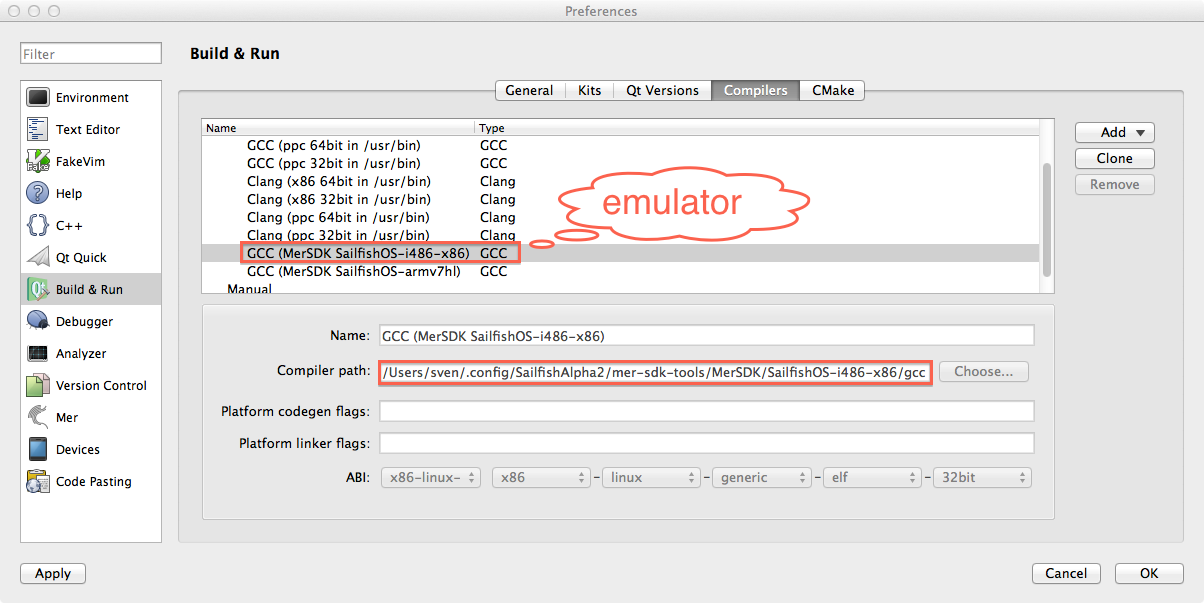
\includegraphics[scale=0.35]{../media/gfx/QtCreator/Compilers.png} 
  \caption{Preferences, compiler tab.}
  \label{fig:creatorcompilers}
\end{figure}
%
The SailfishOS SDK uses GCC as compiler. It is run inside the \nameref{subsec:MerSDK}, see page \pageref{subsec:MerSDK}. Stored on your development machine is only a stub or proxy that wants to connect to the virtual machine and start compiling from there.
%
\begin{figure}[H]
  \centering
  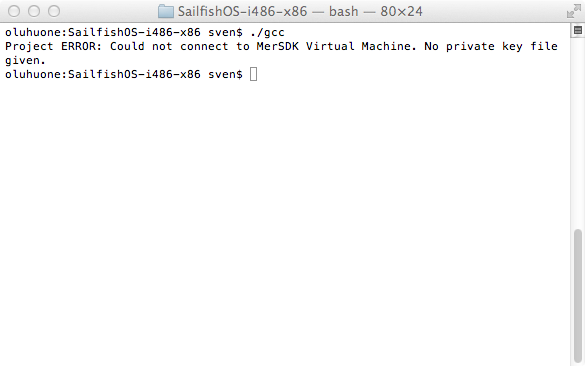
\includegraphics[scale=0.6]{../media/gfx/bash/gcc486.png} 
  \caption{Running GCC from command line.}
  \label{fig:gcc486commandline}
\end{figure}
%
So far I don't know why this piece of software is not installed with the rest of the SDK, \verb, ~/.config, is not a directory where I would expect executables. The error message even shows up if the \textit{Mer build engine for cross compilation} is up and running. Again this helper program is invoked via \nameref{subsubsec:merssh}, see page \pageref{subsubsec:merssh}.

Looking inside \verb,gcc, from the SDK I also find a bash script:
\begin{lstlisting}[language=bash]
#!/bin/bash
exec "/Users/sven/SailfishOS/bin/Qt Creator.app/Contents/MacOS/../Resources/merssh" -sdktoolsdir "/Users/sven/.config/SailfishAlpha3/mer-sdk-tools/MerSDK" -commandtype sb2 -mertarget SailfishOS-i486-x86 gcc $@oluhuone:SailfishOS-i486-x86
\end{lstlisting}
%
\verb,$@, is replaced with the \verb,gcc, call parameters, \verb,oluhuone, is just the name of my current machine.

One questions remains: when is this ever called? To my understanding \verb,qmake, and \verb,make, are called on the \nameref{subsec:MerSDK}. I would conclude that the compiler is invoked from inside the VM.
%
%
\subsubsection{make}\label{subsubsec:make}
%
Again, \verb,make, is just a bash script, \verb,$@, replaced, \verb,oluhuone, my machine:
%
\begin{lstlisting}[language=bash]
#!/bin/bash
exec "/Users/sven/SailfishOS/bin/Qt Creator.app/Contents/MacOS/../Resources/merssh" -sdktoolsdir "/Users/sven/.config/SailfishAlpha3/mer-sdk-tools/MerSDK" -commandtype mb2 -mertarget SailfishOS-i486-x86 make $@oluhuone:SailfishOS-i486-x86
\end{lstlisting}
%
%
I've grepped the command line for the \verb,merssh, while building the application.
%
\begin{lstlisting}[language=bash]
ps -ef|grep "merssh"
\end{lstlisting}
%
Resulting in
%
\begin{lstlisting}[language=bash]
/Users/sven/SailfishOS/bin/Qt Creator.app/Contents/MacOS/../Resources/merssh -sdktoolsdir /Users/sven/.config/SailfishAlpha3/mer-sdk-tools/MerSDK -commandtype mb2 -mertarget SailfishOS-i486-x86 make
\end{lstlisting}
%
Calling \verb,make, on the development machine just calls a proxy script, which forwards the command via \verb,merssh, and executes \verb,make, on the \nameref{subsec:MerSDK}.
%
%
\subsubsection{yaml / spectacle}\label{subsubsec:spectacleyaml}
%
Before the deployment process can build an RPM package of your application, it needs some information about it. This information is provided in the form of \verb,.spec,\footnote{RPM specifications (.spec) files.} text files that are used by the \verb,rpmbuild, program to create the package. If you would do this by hand, you would put the sources into \verb,~/rpmbuild/SOURCES,, the \verb,.spec, named \verb,NAME_OF_THEAPP.spec, into \verb,~/rpmbuild/SPECS, folder, \verb,cd, into it and run
%
\begin{lstlisting}[language=bash]
rpmbuild -ba NAME.spec
\end{lstlisting}
%
to build binary and source packages. Those \verb,.spec, files are also text files but quite hard to read for humans, so in SailfishOS development you will use an intermediate format, called \verb,.yaml,. These contain all the data needed to build a package in a more human friendly presentation. What's inside your \verb,.yaml, depends on your \verb,.pro, file. As a consequence, a new \verb,.yaml, file is built every time you change your \verb.pro. file. The base \verb,.yaml, file of a new SailfishOS QT Quick Application project looks like
%
\begin{lstlisting}[language=tex]
Name:    NAME_OF_THEAPP
Summary: My SailfishOS Application
Version: 0.1
Release: 1
# The contents of the Group field must be one of the groups listed here:
# http://gitorious.org/meego-developer-tools/spectacle/blobs/master/data/GROUPS
Group: Qt/Qt
URL: http://example.org/
License: LICENSE
# This must be generated before uploading a package to a remote build service
Sources:
- '%{name}-%{version}.tar.bz2'
Description: |
  Short description of my SailfishOS Application
Configure: none
# The qtc5 builder inserts macros to allow QtCreator to have fine
# control over qmake/make execution
Builder: qtc5
# Build dependencies should ideally be specified using pkgconfig:
PkgConfigBR:
- sailfishapp >= 0.0.10
- Qt5Core
- Qt5Qml
- Qt5Quick

# Build dependencies without a pkgconfig setup can be listed here
# PkgBR:
#   - package-needed-to-build

# Runtime dependencies which are not automatically detected
Requires:
- sailfishsilica-qt5 >= 0.10.9
# All installed files
Files:
- '%{_datadir}/icons/hicolor/86x86/apps/%{name}.png'
- '%{_datadir}/applications/%{name}.desktop'
- '%{_datadir}/%{name}/qml'
- '%{_bindir}'
# This section is overwritten by Qt Creator. Do not remove the comments.
# Sections ends.
\end{lstlisting}
%
A \verb,.yaml, text file contains information to resolve build and runtime dependencies. First we will see the directives to describe the creation of a \verb,.spec, text file.
%
\emph{Required} - contains the name of the application. That is not the name presented to the user, this is the name of the built binary and its relating files like icons and so on. This should \emph{always} match the \verb,TARGET, declaration in the \verb,.pro, file.
\begin{lstlisting}[language=tex]
Name:
\end{lstlisting}
%
%
\emph{Required} - a short description of your application.
\begin{lstlisting}[language=tex]
Summary:
\end{lstlisting}
%
%
\emph{Required} - the version number of your package\footnote{TODO: what are the conventions? Should this always match the version in the Qt project file?}.
\begin{lstlisting}[language=tex]
Version:
\end{lstlisting}
%
%
This value represents the release version of your RPM package. It is recommended to change this number each time you submit a changed package to the harbour.
\begin{lstlisting}[language=tex]
Release:
\end{lstlisting}
%
%
\emph{Required} - the group in which the application appears in the application launcher. This should always be \verb,Qt/Qt, for a SailfishOS application.
\begin{lstlisting}[language=tex]
Group:
\end{lstlisting}
%
%
\emph{Required} - the name of the license the built package adheres to. This should be the name of the license under which you publish your application.
\begin{lstlisting}[language=tex]
License:
\end{lstlisting}
%
%
\emph{Optional} - a long(er) description of your package/application. The \verb,|, pipe sign means that newlines in the description field shall not be converted into spaces.
\begin{lstlisting}[language=tex]
Description:
\end{lstlisting}
%
%
\emph{Optional} - the name of the tool which was used to build the package. Technically this keyword is optional but you should provide it to prevent warning messages about undefined macro files. Just leave it as it is: \verb,qtc5,.
\begin{lstlisting}[language=tex]
Builder:
\end{lstlisting}
%
%
\emph{Optional} - build dependencies that make use of the assistance of \verb,pkg-config,\cite{fd01}.
\begin{lstlisting}[language=tex]
PkgConfigBR
\end{lstlisting}
%
%
\emph{Optional} - contains the information which packages are needed at runtime. Those packages will be downloaded and installed automatically\footnote{This is true if the package is known in the repositories of your SailfishOS device.} when your this RMP package is installed\footnote{Have a look at the Harbour rules, there are only a few packages available that you can use here.}.
\begin{lstlisting}[language=tex]
Requires:
\end{lstlisting}
%
%
\emph{Optional} - lists the files that are copied to the system when the RPM package is being installed. Each line listed here corresponds to one of the file groups referred to in the \verb,INSTALL, section of your \verb,.prf, or \verb,.pro, file.

\verb,\%{name}, is resolved to the \verb,Name:, entry.
\begin{lstlisting}[language=tex]
Files:
\end{lstlisting}
%
There are some variables or macros that can be used inside a .yaml file\cite{yaml02}:
%
\begin{lstlisting}[language=clean,basicstyle=\ttfamily\tiny]
| Macro             | Typical Expansion    | Meaning                                      |
|:------------------|:---------------------|:---------------------------------------------|
|%{_bindir}	        | /usr/bin	           | Binary directory: where executables are      |
|                   |                      | usually stored.                              |
|%{_builddir}       | ~/rpmbuild/BUILD	   | Build directory: files are compiled within a |
|                   |                      | subdirectory of the build directory.         |
|                   |                      | See %buildsubdir.                            |
|%{buildroot}       | ~/rpmbuild/BUILDROOT | Build root: where files are "installed"      |
|                   |                      | during the %install stage, which copies      |
|                   |                      | files from a subdirectory of %{_builddir}    |
|                   |                      | to a subdirectory of %{buildroot}.           |
|                   |                      | (Historically, %{buildroot} was in           |
|                   |                      | "/var/tmp/".)                                |
|%{buildsubdir}	    | %{_builddir}/%{name} | Build subdirectory: a subdirectory within    |
|                   |                      | %{_builddir} where files are compiled during |
|                   |                      | the %build stage. It is set after %setup.    |
|%{_datadir}        | /usr/share           | Share directory.                             |
|%{_defaultdocdir}  | /usr/share/doc       | Default documentation directory.             |
|%{dist}            | .fcNUMBER	           | Distribution+version short name              |
|                   |                      | (e.g. ".fc20")                               |
|%{fedora} NUMBER   |                      | Number of fedora release (e.g. "20")         |
|%{_includedir}	    | /usr/include         |                                              |
|%{_infodir}        | /usr/share/info      |                                              |
|%{_initrddir}      | /etc/rc.d/init.d     |                                              |
|%{_libdir}	        | /usr/lib             |                                              |
|%{_libexecdir}	    | /usr/libexec         |                                              |
|%{_localstatedir}  | /var                 |                                              |
|%{_mandir}	        | /usr/share/man       |                                              |
|%{name}            |                      | Name of package, set by Name: tag            |
|%{_sbindir}        | /usr/sbin            |                                              |
|%{_sharedstatedir} | /var/lib             |                                              |
|%{_sysconfdir}	    | /etc                 |                                              |
|%{version}         |                      | Version of package, set by Version: tag      |
\end{lstlisting}
%
As you can see, not everything makes sense in the SailfishOS environment.
%
%
\subsubsection{pkg-config}\label{subsubsec:pkgconfig}
%
\begin{lstlisting}[language=bash]
pkg-config --list-all
\end{lstlisting}
%
Works just in the scratch box environment; TODO
%
%
\subsubsection{rpm}\label{subsubsec:rpm}
%
Red Hat Package Manager or RPM Package Manager (RPM) is a package management system.[4] The name RPM variously refers to the .rpm file format, files in this format, software packaged in such files, and the package manager itself. RPM was intended primarily for Linux distributions; the file format is the baseline package format of the Linux Standard Base\cite{wiki03}.

Guess what, the command is a bash script inside the SDK:
%
\begin{lstlisting}[language=bash]
#!/bin/bash
exec "/Users/sven/SailfishOS/bin/Qt Creator.app/Contents/MacOS/../Resources/merssh" -sdktoolsdir "/Users/sven/.config/SailfishAlpha3/mer-sdk-tools/MerSDK" -commandtype mb2 -mertarget SailfishOS-i486-x86 rpm $@oluhuone:SailfishOS-i486-x86
\end{lstlisting}
%
This script is called when you \verb,deploy, your app. Deploying happens implicitly if you \emph{run} the application. See section \nameref{subsubsec:runsettings} on page \pageref{subsubsec:runsettings}. Or you can deploy explicitly.

Here are some useful commands, we are examining the package \verb,qt5-qtcore,.

\begin{lstlisting}[language=bash]
[root@SailfishSDK ~]# rpm -q qt5-qtcore
# shows package version number
\end{lstlisting}
%
\begin{lstlisting}[language=bash]
[root@SailfishSDK ~]# rpm -ql qt5-qtcore
# shows all the files contained in the package qt5-qtcore
\end{lstlisting}
%
\begin{lstlisting}[language=bash]
[root@SailfishSDK ~]# rpm -qR qt5-qtcore
# shows package dependencies
\end{lstlisting}

%
%
\subsubsection{deploy}\label{subsubsec:deploy}
%
There are two ways to start the deployment process, also have a look at  section \nameref{subsubsec:runsettings} on page \pageref{subsubsec:runsettings}.
%
\begin{figure}[H]
  \centering
  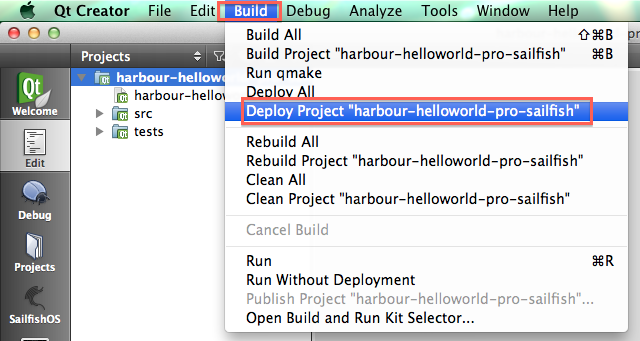
\includegraphics[scale=0.5]{../media/gfx/QtCreator/deploy01-01.png} 
  \caption{Deploy via ``build'' menu.}
  \label{fig:deploy01-01}
\end{figure}
%
% 
\begin{figure}[H]
  \centering
  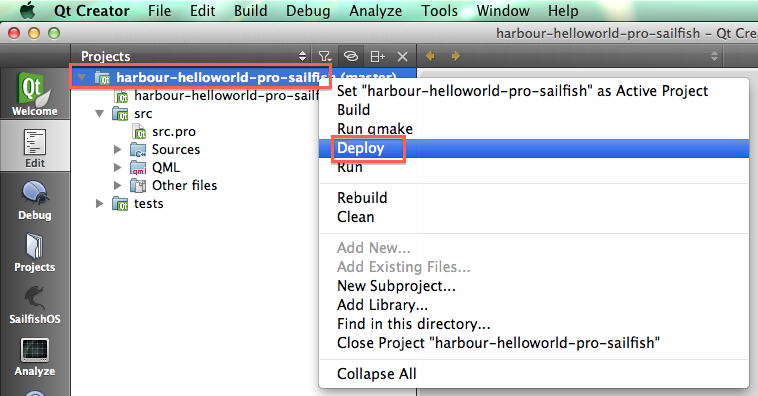
\includegraphics[scale=0.5]{../media/gfx/QtCreator/deploy01-02.png} 
  \caption{Deploy via ``project tree''.}
  \label{fig:deploy01-02}
\end{figure}
%
%
\subsubsection{Project settings}\label{subsubsec:projectsettings}
%
As so often in life there is more than one way to do things. There are the $\vbox{\hbox{
\includegraphics[scale=0.4]{../media/gfx/QtCreator/projects.png}}}$ \emph{project settings}. This is the place where you define what happens when you build and compile.
% 
\begin{figure}[H]
  \centering
  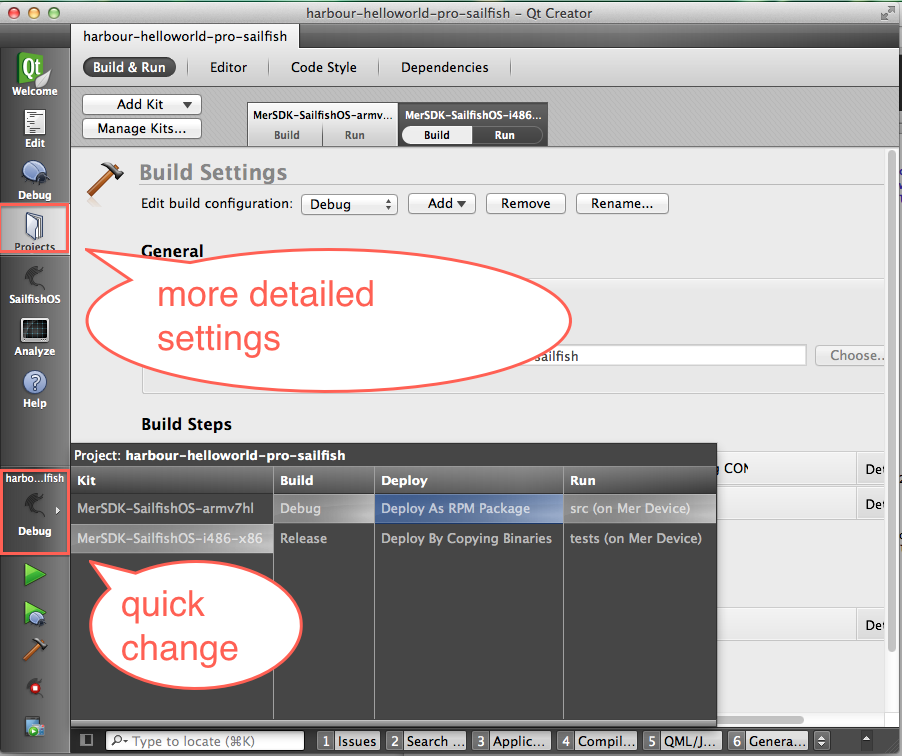
\includegraphics[scale=0.5]{../media/gfx/QtCreator/ProjectSettings01.png} 
  \caption{Two way to change project settings.}
  \label{fig:ProjectSettings01}
\end{figure}
%
The second way is the fast \emph{mode selector} $\vbox{\hbox{
\includegraphics[scale=0.4]{../media/gfx/QtCreator/ModeSelector.png}}}$ that switches between the settings that were defined in the \emph{project settings}. It's the sailfish button above the green run button.
%
%
You have started a project just with the \verb,SailfishOS-i486-x86, setting\footnote{Or vice versa.} or meanwhile there is another platform available. In any of those cases the $\vcenter{\hbox{
\includegraphics[scale=0.6]{../media/gfx/QtCreator/addkitbutton.png}}}$ button is your way to go. This way you can add new target platforms. In Qt-Speak they are called \nameref{subsubsec:kits}, a combination of Qt library, compiler and deployment target.

Right next to it is a little section for each platform you have chosen to build for. Each of this sections is decided into a \emph{build} and \emph{run} pane. As you can guess, \emph{build} defines how to build your app, \emph{run} defines how to run it.
% 
\begin{figure}[H]
  \centering
  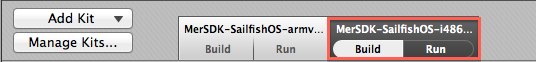
\includegraphics[scale=0.6]{../media/gfx/QtCreator/kitbuildrun.png} 
  \caption{Settings for build and run for each target.}
  \label{fig:kitbuildrun}
\end{figure}
%
%
\subsubsection{Build settings}\label{subsubsec:buildsettings}
%
Do you want to build a \verb,debug, version of your app with all the debug symbol built-in? Or are you ready to ship your app to the \nameref{sec:harbour}?
%
\begin{figure}[H]
  \centering
  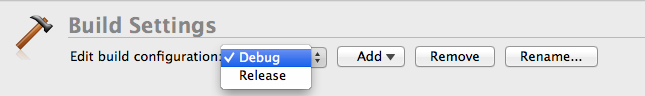
\includegraphics[scale=0.6]{../media/gfx/QtCreator/DebugRelease.png} 
  \caption{Build Debug or Release version?.}
  \label{fig:DebugRelease}
\end{figure}
%
The build directory of your app can but must not be the same as your source directory\footnote{Shadow builds work since the Alpha3 SDK.}. If you check ``Shadow build'', the code will be built in another directory (for each kit). This way you do not need to \verb,make clean, after changing between the targets.
%
\begin{figure}[H]
  \centering
  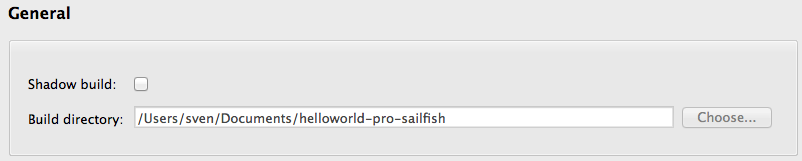
\includegraphics[scale=0.5]{../media/gfx/QtCreator/GeneralBuildDirectory.png} 
  \caption{Where should your code be built?.}
  \label{fig:GeneralBuildDirectory}
\end{figure}
%
The \nameref{subsec:mersdkpkg} has mounted your home drive and eventually a separate source code directory from your development machine. So don't wonder why the build directory is local on your machine?

The \emph{Build steps} section defines what happens if you actually build your app. If you open up the details, you can see the called command line.
%
\begin{figure}[H]
  \centering
  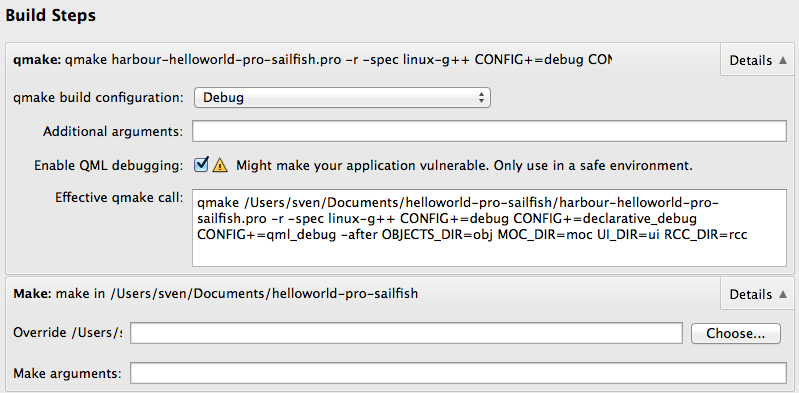
\includegraphics[scale=0.5]{../media/gfx/QtCreator/BuildSteps.png} 
  \caption{How to build?.}
  \label{fig:BuildSteps}
\end{figure}
%
Usually \nameref{subsubsec:qmake} is called, followed by \nameref{subsubsec:make}. \emph{Note}: those commands are not invoked locally, they run remote on the \nameref{subsec:MerSDK}, as defined in the preferences for the QtCreator\footnote{Preferences->bash scripts->merssh->VM}.

\emph{Clean steps} defines how your project is \verb,make clean,ed.
%
\begin{figure}[H]
  \centering
  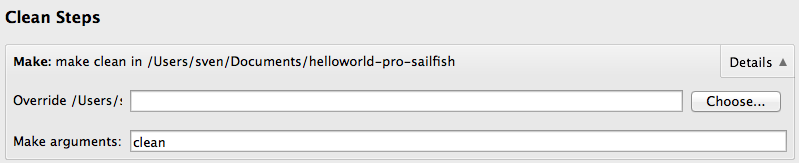
\includegraphics[scale=0.5]{../media/gfx/QtCreator/CleanSteps.png} 
  \caption{How to clean your project?.}
  \label{fig:CleanSteps}
\end{figure}
%

The \emph{Build environment} defines the environment variables that are used during build.
%
%
\subsubsection{Pimp the clean process}\label{subsubsec:pimpclean}
%
Every now and then you clean your project. What bugged my for some time using QtCreator\footnote{That has nothing to do with the SailfishOS SDK, the regular QtCreator does that, too.} was that it left the Makefile after you cleaned the project. This way \verb,qmake, is often not run after a \verb,make clean,. No problem, just choose the \emph{\nameref{subsubsec:buildsettings}} pane of the \emph{project settings} and hit the button $\vcenter{\hbox{
\includegraphics[scale=0.6]{../media/gfx/QtCreator/addcleanstep.png}}}$ and create an extra step that is executed every time after the cleanup has been done.
%
\begin{figure}[H]
  \centering
  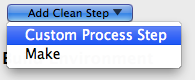
\includegraphics[scale=0.6]{../media/gfx/QtCreator/customprocessstep.png} 
  \caption{Create a custom process step.}
  \label{fig:customprocessstep}
\end{figure}
%
%
\begin{figure}[H]
  \centering
  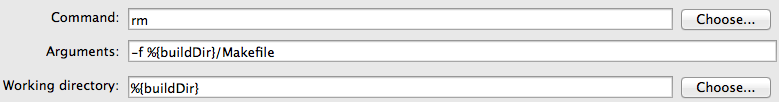
\includegraphics[scale=0.55]{../media/gfx/QtCreator/rmMakefile.png} 
  \caption{Clean step: Remove the Makefile.}
  \label{fig:rmMakefile}
\end{figure}
%
Here again for copy and paste:
\begin{lstlisting}[language=bash]
rm
-f %{buildDir}/Makefile
%{buildDir}
\end{lstlisting}
%
%
\subsubsection{Run settings}\label{subsubsec:runsettings}
%
Here you have some control on how the compiled binary and its companion files will be transferred to the target device.

Choose \emph{Deploy By Copying Binaries} if you are in an early development stage and recompile very often. It's the faster way.
%
\begin{figure}[H]
  \centering
  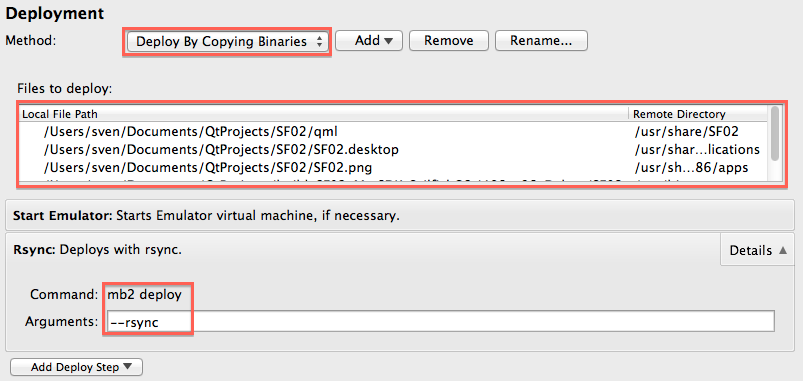
\includegraphics[scale=0.5]{../media/gfx/QtCreator/RunSettingsCopyBinary.png} 
  \caption{Run Setting, Deploy By Copying Binaries.}
  \label{fig:RunSettingsCopyBinary}
\end{figure}
%
If your app is almost ready to ship to the \nameref{sec:harbour}, you can change to \emph{RPM}. Now your binary and resource files will be packaged into a RPM file, transferred to the target device and installed like any other application from the store. As RPM packages can contain dependencies to other packages, you can profit from an automatic installation of those packages you depend on\footnote{Have a look at section \nameref{sec:harbour} on page \pageref{sec:harbour} which other packages are allowed or the other way around: which packages are not blacklisted}.
%
\begin{figure}[H]
  \centering
  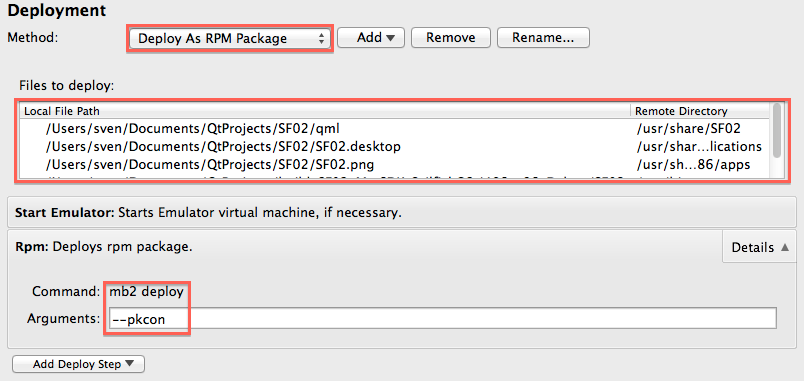
\includegraphics[scale=0.5]{../media/gfx/QtCreator/RunSettingsRpm.png} 
  \caption{Run Setting, Deploy As RPM Package.}
  \label{fig:RunSettingsRpm}
\end{figure}
%
\emph{Files to deploy} show which files from your computer go where on the target device.
Either way uses a variation of the \verb,mb2 deploy, command on the \nameref{subsec:MerSDK}, which means that the binaries or packages are transferred from one VM to the other VM.

The \emph{Run configuration} contains information about how your app is run on the target device.
%
\begin{figure}[H]
  \centering
  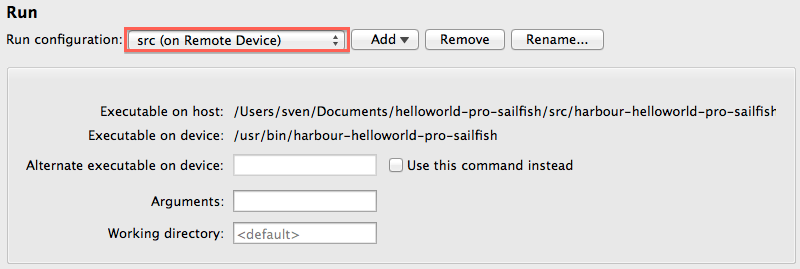
\includegraphics[scale=0.5]{../media/gfx/QtCreator/RunSettings.png} 
  \caption{Run configuration.}
  \label{fig:RunSettings}
\end{figure}
%
In case your project consists of more than one (sub-)project, the \emph{configuration} determines which of these should run. \emph{Executable on host} is the path to the compiled binary locally on your development machine. In contrast is the \emph{Executable on device} the path to the transferred binary on the target device\footnote{If you hit \emph{run}, the binary is copied or installed at his location.}.

The \emph{Run environment} represents the environment variables that are visible to the binary when it is executed on the target device.
%
\begin{figure}[H]
  \centering
  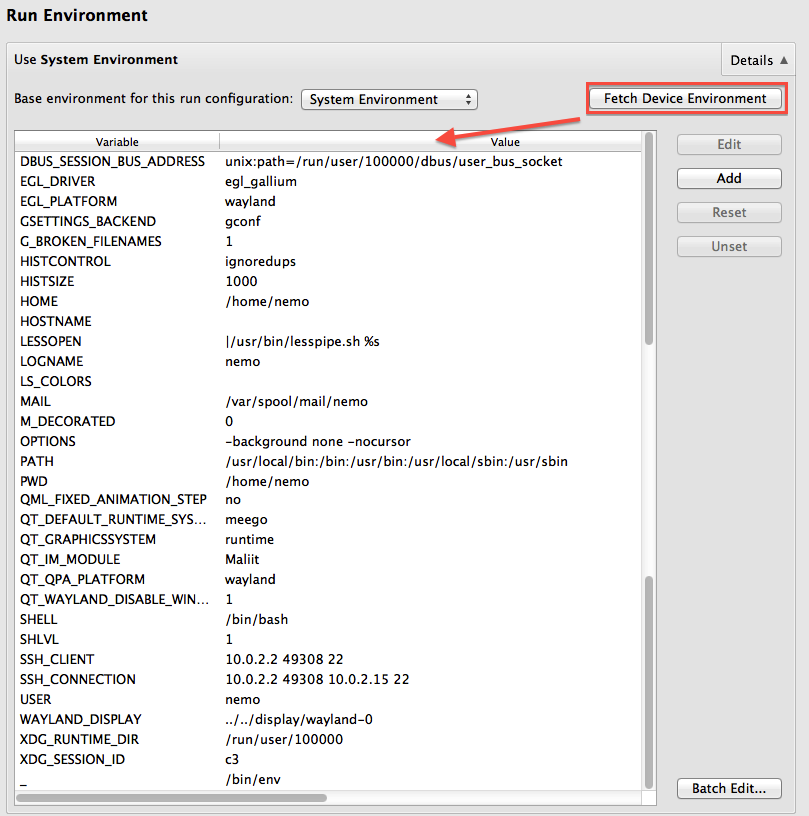
\includegraphics[scale=0.55]{../media/gfx/QtCreator/RunEnvironment.png} 
  \caption{Run environment - environment variables on target device.}
  \label{fig:RunEnvironment}
\end{figure}
%
To see them, you must start the emulator and click on the $\vcenter{\hbox{
\includegraphics[scale=0.6]{../media/gfx/QtCreator/FetchDeviceEnvironmentButton.png}}}$ button.
%
The \emph{Analyzer Settings} are clearly for \verb,valgrind, a static analyzer tool. I haven't used it one the emulator yet and on OSX Mountain Lion it does not run anymore. I'd prefer \verb,clang, which is AFAIK not available on the SDK.

The \emph{Debugger Settings} are for TODO (the checkboxes are pretty cleat that it's about switching debugger support on and off but I haven't used it in this environment so far - so I don't make things up here).
%

You can use 2 variables inside the parameters for build/run settings:
%
\begin{itemize}
\item \verb,%{buildDir},
\item \verb,%{sourceDir},
\end{itemize}
%
%
\subsection{Mer build engine for cross compilation}\label{subsec:MerSDK}
%
``The Mer build engine is a virtual machine (VM) containing the Mer development toolchains and tools. It also includes a SailfishOS target for building and running Sailfish and QML applications. The target is mounted as a shared folder to allow QtCreator to access the compilation target. Additionally, your home directory is shared and mounted in the VM, thus giving access to your source code for compilation.
The build engine also supports additional build targets and cross-compilation toolchains. These can be managed from the SDK Control Centre interface within QtCreator which allows toolchains, targets and even individual target packages to be added and removed.''\cite{sailfishos3}.
%
\begin{figure}[H]
  \centering
  
\includegraphics[scale=0.5]{../media/gfx/QtCreator/MerSDKsettings.png} 
  \caption{SailfishOS icon.}
  \label{fig:creatormersdkicon}
\end{figure}
%
The VM runs headless\footnote{You can change that in Preferences->Mer, uncheck "Headless" and restart the VM or start in from the VirtualBox control center of you need it just once.}, you can not see it running. For you as a developer there is a webpage served by this VM accessible through the SailfishOS icon inside QtCreator. See figure \ref{fig:managesdkupdate} on page \pageref{fig:managesdkupdate}.
%
\begin{figure}[H]
  \centering
  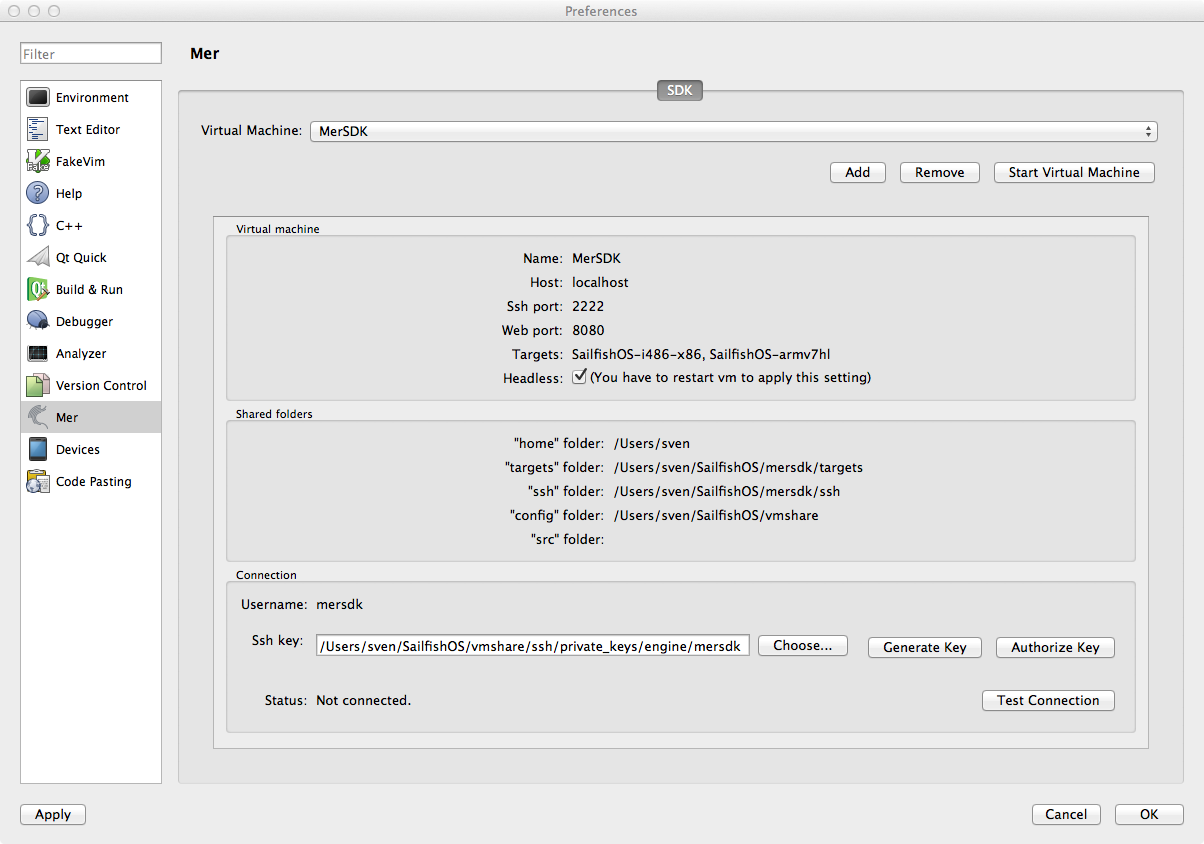
\includegraphics[scale=0.3]{../media/gfx/QtCreator/MerSDK.png} 
  \caption{Preferences, Mer SDK - virtual machine.}
  \label{fig:creatormersdk}
\end{figure}
%
%
\subsubsection{Directories}\label{subsubsec:mersdkdirectories}
%
VirtualBox shared folders are used for sharing files between the host and the build engine and emulators\cite{mer04}:
\begin{itemize}
\item Configuration
\item SSH keys
\item Home directory
\item Targets
\item Other source directory trees
\end{itemize}
%
\begin{figure}[H]
  \centering
  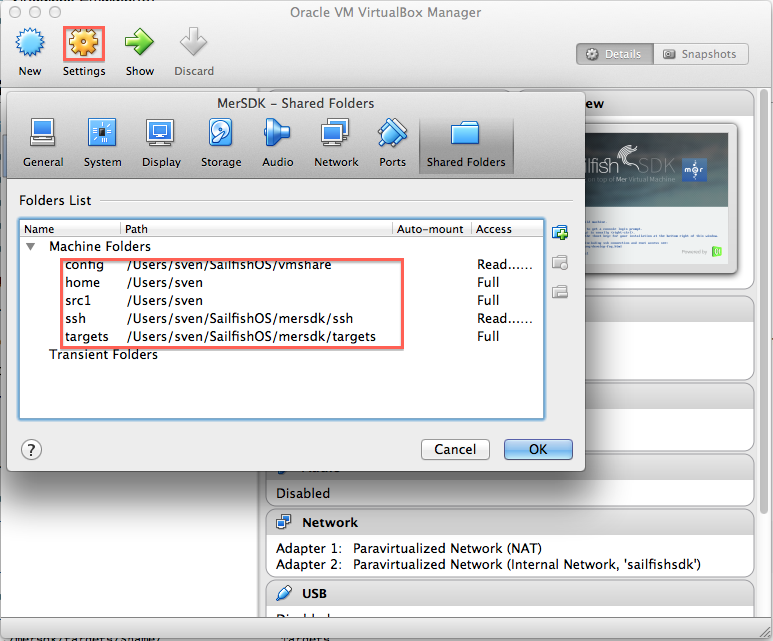
\includegraphics[scale=0.5]{../media/gfx/VirtualBox/vboxMerSettings02.png} 
  \caption{Virtual Box, shared folders.}
  \label{fig:vboxMerSettings02}
\end{figure}
%
Those shared folders are mount to these positions in the filesystem of the Mer build engine for cross compilation:
\begin{lstlisting}[language=bash]
[root@SailfishSDK ~]# mount
none on /etc/ssh/authorized_keys type vboxsf (rw,nodev,relatime)
none on /home/mersdk type vboxsf (rw,nodev,relatime)
none on /host_targets type vboxsf (rw,nodev,relatime)
none on /etc/mersdk/share type vboxsf (rw,nodev,relatime)
none on /home/src1 type vboxsf (rw,nodev,relatime)
\end{lstlisting}

You can also see those and many other settings on the command line via the \verb,VBoxManage, command.
\begin{lstlisting}[language=bash]
VBoxManage showvminfo "MerSDK"
\end{lstlisting}
%
%
\subsection{Scratchbox2}\label{subsec:scratchbox2}
%
``Scratchbox2 (sbox2 or sb2) is a cross-compilation toolkit designed to make embedded Linux application development easier. It also provides a full set of tools to integrate and cross-compile an entire Linux distribution.

In the Linux world, when building software, many parameters are auto-detected based on the host system (like installed libraries and system configurations), through autotools "./configure" scripts for example. But so, when one wants to build for an embedded target (cross-compilation), most of the detected parameters are incorrect (i.e. host configuration is not the same as the embedded target configuration).

Without Scratchbox2, one has to manually set many parameters and "hack" the "configure" process to be able to generate code for the embedded target.

At the opposite, Scratchbox2 allows one to set up a "virtual" environment that will trick the autotools and executables into thinking that they are directly running on the embedded target with its configuration.

Moreover, Scratchbox2 provides a technology called CPU-transparency that goes further in that area. With CPU-transparency, executables built for the host CPU or for the target CPU could be executed directly on the host with sbox2 handling the task to CPU-emulate if needed to run a program compiled for the target CPU. So, a build process could mix the usage of program built for different CPU architectures. That is especially useful when a build process requires building the program X to be able to use it to build the program Y (Example: building a Lexer that will be used to generate code for a specific package).''\cite{wiki02}

The Wiki page of the Mer project contains a exhaustive description how to compile a program on platform A for platform B\cite{mer01}.
%
\subsubsection{sb2}\label{subsubsec:sb2}
%
You can find Scratchbox2 or the \verb,sb2, in the \verb,/usr/bin, folder of the \nameref{subsec:MerSDK}. This shell script is not called directly. The SailfishOS SDK uses \nameref{subsubsec:mb2} as a wrapper for convenience.
%
%
\subsubsection{mb2}\label{subsubsec:mb2}
%
This is a convenience wrapper script in the \verb,/usr/bin, folder of the \nameref{subsec:MerSDK}.. Look at the source code in section \nameref{subsec:appendix:mb2} on page \pageref{subsec:appendix:mb2}.

Here is just the usage part to grab what is happening when this script is called\footnote{It should be alright to show a snippet since I included the whole source with copyright notice.}.
%
\begin{lstlisting}[language=bash]
  Executes a subset of build commands in the context of an rpmbuild.
  Typically called from QtCreator to perform qmake/make phases of a project.
  Note that any other build steps in the .spec file will also be run.

  <specfile> will be looked for in the current rpm/ dir. If there is
  more than one it must be provided.

  CWD is used as a base dir for installroot/ and RPMS/ to allow for
  shadowbuilds

  mb2 is aware of spectacle and will update the spec file if there is
  an obvious yaml file which is newer.

  mb2 build [-d] [-j <n>] [<args>]
                     : runs rpmbuild for the given spec file in the
                       given sb2 target. Produces an rpm package.
                     : -d     enable debug build
                     : -j <n> use only 'n' CPUs to build
                     : can use -s -t -p

  mb2 qmake [<args>] : runs qmake in the 'build' phase
                       Note that this also verifies target
                       build dependencies are up to date
                     : can use -s -t -p  

  mb2 make [<args>]  : run make in the 'build' phase
                     : can use -s -t -p  

  mb2 deploy \textendashzypper|--pkcon|--rsync
                     : runs the install or rpm-creation phase and then
                       copies/installs the relevant files to the device
                     : can use -s -t -p -d

  mb2 run|ssh [<args>] : runs a command (on device if --device given);
                         intended for running gdb and a gdb server
                     : can use -s -t -p -d

  mb2 install [<args>] : runs the 'install' phase to install to $buildroot
                     : can use -s -t -p
  mb2 rpm [<args>]   : runs the install & rpm-creation phases
                     : can use -s -t -p


  -t | --target      : specify the sb2 target to use
  -d | --device      : specify the device
  -p | --projectdir  : when running shadow build/deploy from another dir
  -s | --specfile    : if the specfile is not in rpm/*.spec and cannot be found using -p
\end{lstlisting}
%
%
\subsection{The SailfishOS Emulator}\label{subsec:SailfishEmulator}
%
``The emulator is an x86 VM image containing a stripped down version of the target device software. It emulates most of the functions of the target device running Sailfish operating system, such as gestures, task switching and ambience theming.''\cite{sailfishos3}.
At least with the AlphaSDK3 the emulator can not simulate device rotations.
%
\begin{figure}[H]
  \centering
  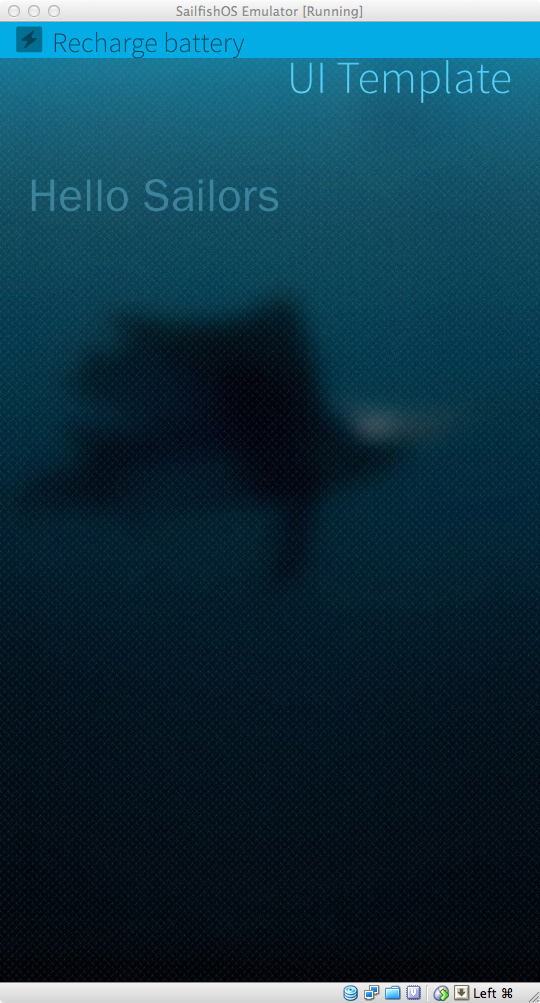
\includegraphics[scale=0.3]{../media/gfx/emulator/emulatorexample.png} 
  \caption{Emulator running the templated SailfishOS Qt Quick Application.}
  \label{fig:emulatorexample}
\end{figure}
%
The Alpha3 SDK emulator brought new settings for developers.

Choose
$\vcenter{\hbox{
\includegraphics[scale=0.3]{../media/gfx/emulator/developerSettings01-01.png}}}$, tap on
$\vcenter{\hbox{
\includegraphics[scale=0.3]{../media/gfx/emulator/developerSettings01-02.png}}}$ and then
$\vcenter{\hbox{
\includegraphics[scale=0.3]{../media/gfx/emulator/developerSettings01-03.png}}}$ \\
%
Finally in the developer settings you can choose a password for the user \verb,nemo, or update the package repositories.
%
\begin{figure}[H]
  \centering
  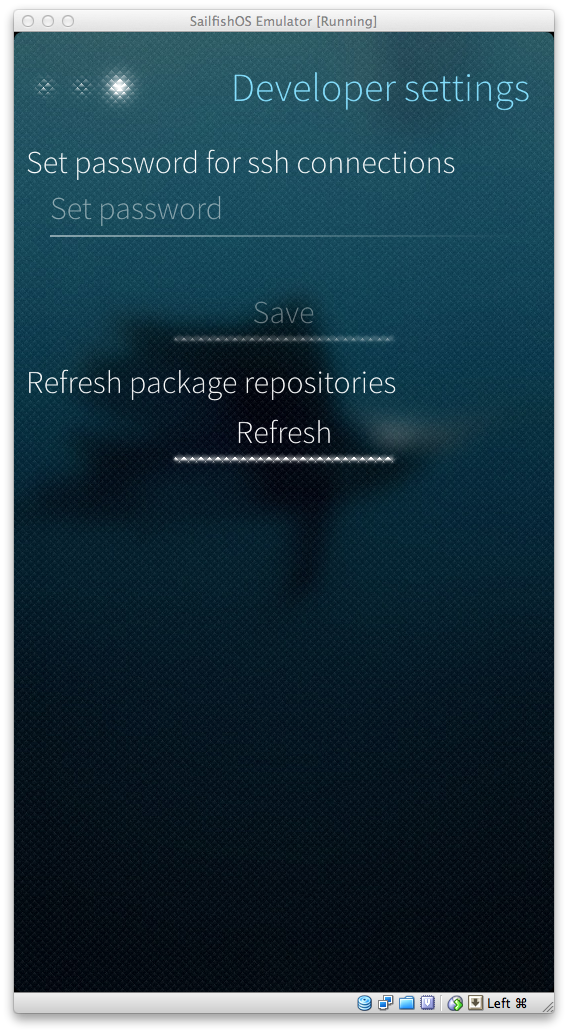
\includegraphics[scale=0.3]{../media/gfx/emulator/developerSettings01-04.png} 
  \caption{Choose password or update package repositories.}
  \label{fig:developerSettings01-04}
\end{figure}
%
%
\subsection{Sailfish Silica}\label{subsec:SailfishSilica}
%
``Sailfish Silica is a QML module which provides Sailfish UI components for applications. Their look and feel fits with the Sailfish visual style and behavior and enables unique Sailfish UI application features, such as pulley menus and application covers.''\cite{sailfishos3}.

QML\cite{qt05} is the Qt \emph{Q}uick \emph{M}arkup \emph{L}anguage\cite{qt06} that supersedes widgets for designing user interfaces. It is a declarative ``language'' that can contain a small subset of Javascript.
%

Also have a look at some open source examples on Github\cite{sailfishos5}.
The emulator comes with a demo application that shows the silica components.
%
\begin{figure}[H]
\centering
\subfloat{
  \centering
  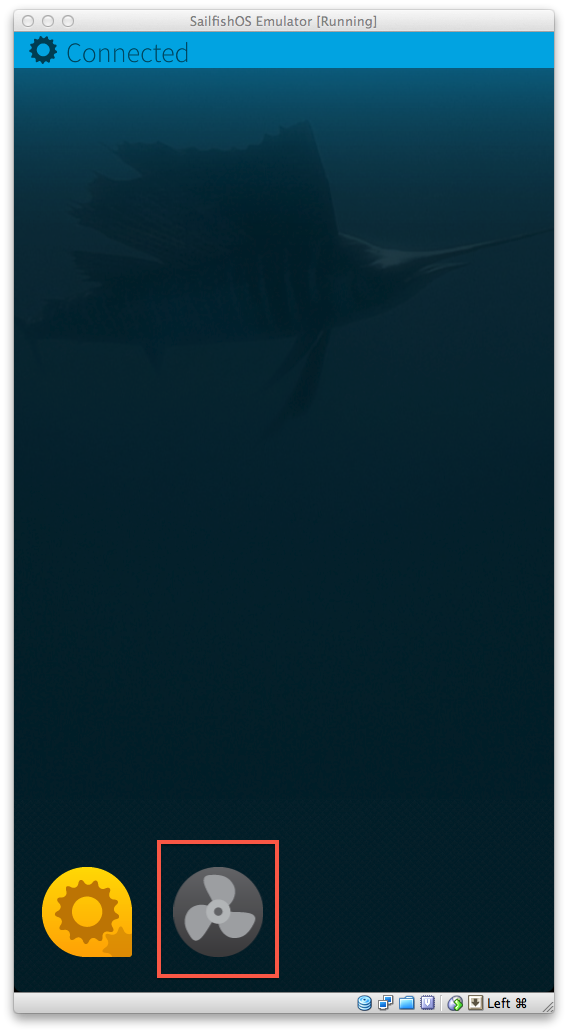
\includegraphics[scale=0.3]{../media/gfx/silica/silica01.png}
  \label{fig:silica01}
}%
\subfloat{
  \centering
  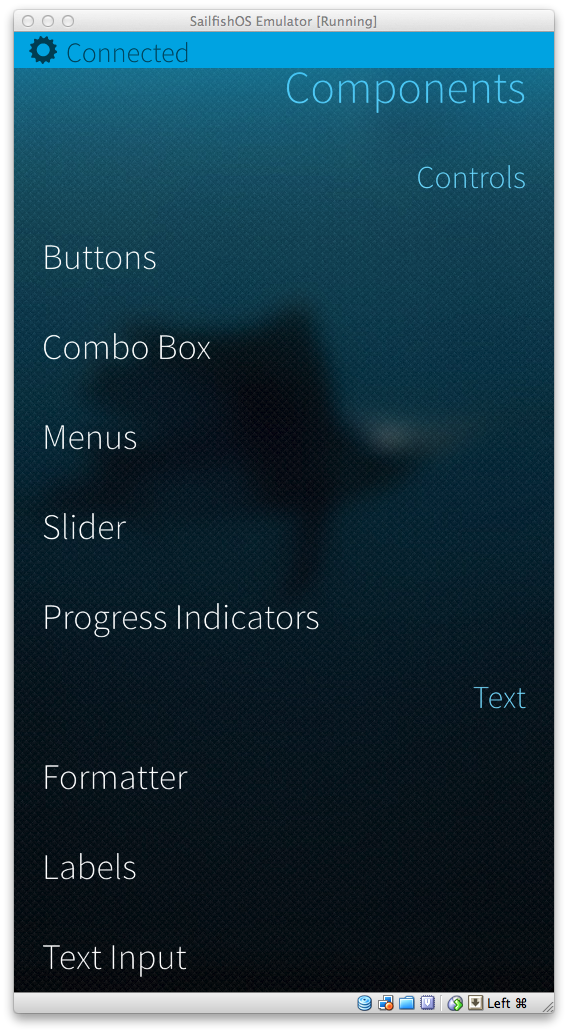
\includegraphics[scale=0.3]{../media/gfx/silica/silica02.png}
  \label{fig:silica02}
}
\end{figure}
%
\begin{figure}[H]
\centering
\subfloat{
  \centering
  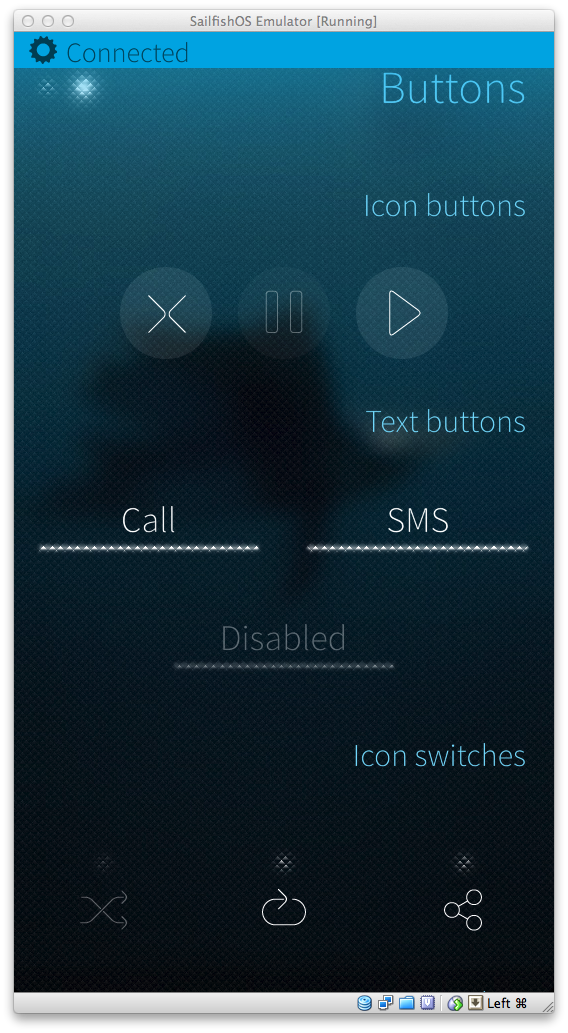
\includegraphics[scale=0.3]{../media/gfx/silica/silica03.png}
  \label{fig:silica03}
}%
\subfloat{
  \centering
  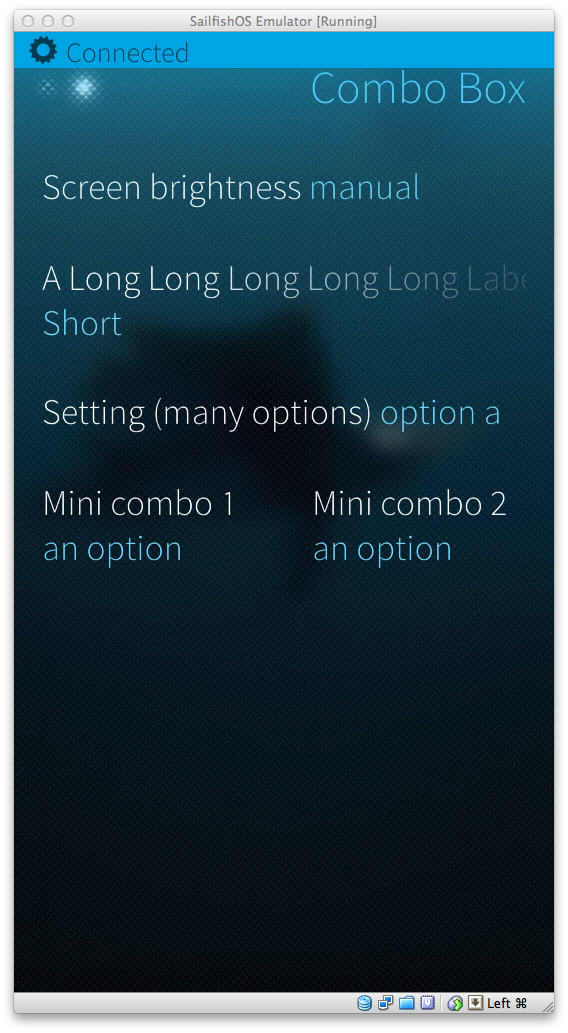
\includegraphics[scale=0.3]{../media/gfx/silica/silica04.png}
  \label{fig:silica04}
}
\end{figure}
%
\begin{figure}[H]
\centering
\subfloat{
  \centering
  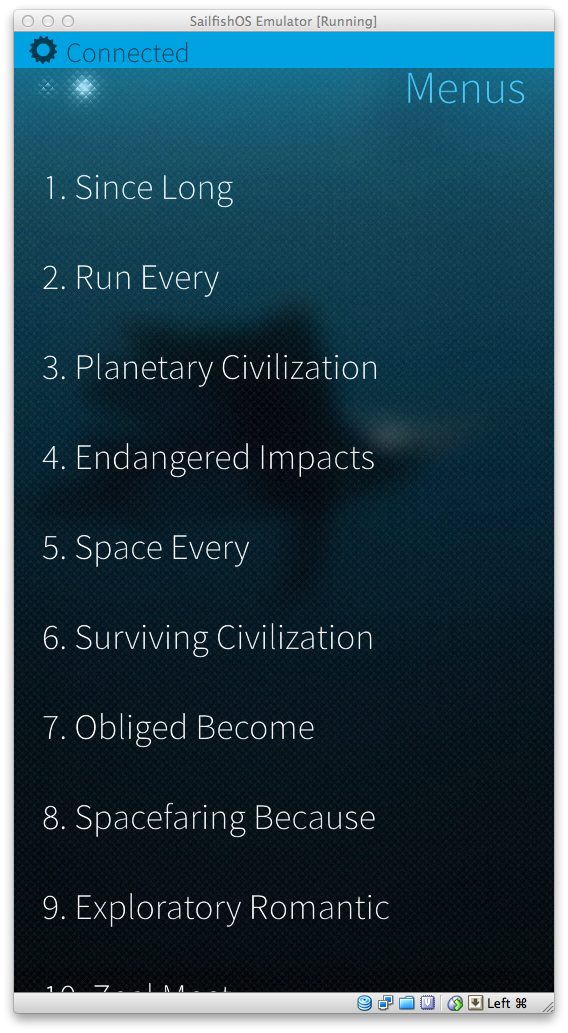
\includegraphics[scale=0.3]{../media/gfx/silica/silica05.png}
  \label{fig:silica05}
}%
\subfloat{
  \centering
  \includegraphics[scale=0.3]{../media/gfx/silica/silica06.png}
  \label{fig:silica06}
}
\end{figure}
%
\begin{figure}[H]
\centering
\subfloat{
  \centering
  \includegraphics[scale=0.3]{../media/gfx/silica/silica07.png}
  \label{fig:silica07}
}%
\subfloat{
  \centering
  \includegraphics[scale=0.3]{../media/gfx/silica/silica08.png}
  \label{fig:silica08}
}
\end{figure}
%
\begin{figure}[H]
\centering
\subfloat{
  \centering
  \includegraphics[scale=0.3]{../media/gfx/silica/silica09.png}
  \label{fig:silica09}
}%
\subfloat{
  \centering
  \includegraphics[scale=0.3]{../media/gfx/silica/silica10.png}
  \label{fig:silica10}
}
\end{figure}
%
%
\subsection{Tools chained up}\label{subset:toolschainedup}
%
Now that we have seen all the tools, bits and pieces, I will try to give an overview how everything works together, when you compile your code in QtCreator for SailfishOS.
%
%
\subsubsection{Build process}\label{subsubsec:buildprocess}
%
As an example we just assume that the user\footnote{That means you ;-)} builds an app for the emulator and thus uses the \verb,SailfishOS-i486-x86, target.
\\
\\
\begin{tabular}{l|l|l}
  \emph{QtCreator} & \emph{Mer SDK VM} & \emph{emulator} \\ \hline
  %
  \parbox[t]{0.33\textwidth}{user starts build} &
  \parbox[t]{0.33\textwidth}{} &
  \parbox[t]{0.33\textwidth}{} \\ \hline
  %
  \parbox[t]{0.33\textwidth}{qmake} &
  % ~/.config/SailfishAlpha3/mer-sdk-tools/MerSDK/SailfishOS-i486-x86/qmake
  \parbox[t]{0.33\textwidth}{} &
  \parbox[t]{0.33\textwidth}{} \\ \hline
  %
  \parbox[t]{0.33\textwidth}{merssh} &
  \parbox[t]{0.33\textwidth}{} &
  \parbox[t]{0.33\textwidth}{} \\ \hline
  %
  \parbox[t]{0.33\textwidth}{} &
  \parbox[t]{0.33\textwidth}{mb2 -mertarget SailfishOS-i486-x86 qmake} &
  \parbox[t]{0.33\textwidth}{} \\ \hline
  %
  \parbox[t]{0.33\textwidth}{make} &
  % ~/.config/SailfishAlpha3/mer-sdk-tools/MerSDK/SailfishOS-i486-x86/make
  \parbox[t]{0.33\textwidth}{} &
  \parbox[t]{0.33\textwidth}{} \\ \hline
  %
  \parbox[t]{0.33\textwidth}{merssh} &
  \parbox[t]{0.33\textwidth}{} &
  \parbox[t]{0.33\textwidth}{} \\ \hline
  %
  \parbox[t]{0.33\textwidth}{} &
  \parbox[t]{0.33\textwidth}{mb2 -mertarget SailfishOS-i486-x86 make} &
  \parbox[t]{0.33\textwidth}{} \\ \hline
  %
  \parbox[t]{0.33\textwidth}{parse output} &
  \parbox[t]{0.33\textwidth}{} &
  \parbox[t]{0.33\textwidth}{} \\ \hline  
\end{tabular} \\
%
%
\subsubsection{Run app}\label{subsubsec:runapp}
%
Now the user hits \emph{run}, variation 1 = \emph{Deploy By Copying Binaries}.
\\
\\
\begin{tabular}{l|l|l}
  \emph{QtCreator} & \emph{Mer SDK VM} & \emph{emulator} \\ \hline
  %
  \parbox[t]{0.33\textwidth}{user runs app} &
  \parbox[t]{0.33\textwidth}{} &
  \parbox[t]{0.33\textwidth}{} \\ \hline
  %
  \parbox[t]{0.33\textwidth}{start emulator if necessary} &
  \parbox[t]{0.33\textwidth}{} &
  \parbox[t]{0.33\textwidth}{} \\ \hline
  %
  \parbox[t]{0.33\textwidth}{deploy} &
  \parbox[t]{0.33\textwidth}{} &
  \parbox[t]{0.33\textwidth}{} \\ \hline

  %
  \parbox[t]{0.33\textwidth}{merssh} &
  \parbox[t]{0.33\textwidth}{} &
  \parbox[t]{0.33\textwidth}{} \\ \hline
  %
  \parbox[t]{0.33\textwidth}{} &
  \parbox[t]{0.33\textwidth}{mb2 -mertarget SailfishOS-i486-x86 deploy --rsync\footnote{TODO examine the steps, there has to be a make install inside.}} &
  \parbox[t]{0.33\textwidth}{} \\ \hline
  %
  \parbox[t]{0.33\textwidth}{} &
  \parbox[t]{0.33\textwidth}{copying files to the emulator} &
  \parbox[t]{0.33\textwidth}{} \\ \hline
  %
  \parbox[t]{0.33\textwidth}{run executable on remote device} &
  \parbox[t]{0.33\textwidth}{} &
  \parbox[t]{0.33\textwidth}{} \\ \hline
  %
  \parbox[t]{0.33\textwidth}{} &
  \parbox[t]{0.33\textwidth}{} &
  \parbox[t]{0.33\textwidth}{execute binary} \\ \hline
  %
  \parbox[t]{0.33\textwidth}{catch execution status} &
  \parbox[t]{0.33\textwidth}{} &
  \parbox[t]{0.33\textwidth}{} \\ \hline
\end{tabular} \\
\\
\\
%
%
Or the user hits \emph{run}, variation 2 = \emph{Deploy As RPM Package}.
\\
\\
\begin{tabular}{l|l|l}
  \emph{QtCreator} & \emph{Mer SDK VM} & \emph{emulator} \\ \hline
  %
  \parbox[t]{0.33\textwidth}{user runs app} &
  \parbox[t]{0.33\textwidth}{} &
  \parbox[t]{0.33\textwidth}{} \\ \hline
  %
  \parbox[t]{0.33\textwidth}{start emulator if necessary} &
  \parbox[t]{0.33\textwidth}{} &
  \parbox[t]{0.33\textwidth}{} \\ \hline
  %
  \parbox[t]{0.33\textwidth}{deploy} &
  \parbox[t]{0.33\textwidth}{} &
  \parbox[t]{0.33\textwidth}{} \\ \hline
  %
  \parbox[t]{0.33\textwidth}{merssh} &
  \parbox[t]{0.33\textwidth}{} &
  \parbox[t]{0.33\textwidth}{} \\ \hline
  %
  \parbox[t]{0.33\textwidth}{} &
  \parbox[t]{0.33\textwidth}{mb2 -mertarget SailfishOS-i486-x86 deploy --pkcon} &
  \parbox[t]{0.33\textwidth}{} \\ \hline
  %
  \parbox[t]{0.33\textwidth}{} &
  \parbox[t]{0.33\textwidth}{building RPM package} &
  \parbox[t]{0.33\textwidth}{} \\ \hline
  %
  \parbox[t]{0.33\textwidth}{} &
  \parbox[t]{0.33\textwidth}{copying RPM package to the emulator} &
  \parbox[t]{0.33\textwidth}{} \\ \hline
  %
  \parbox[t]{0.33\textwidth}{} &
  \parbox[t]{0.33\textwidth}{} &
  \parbox[t]{0.33\textwidth}{installing RPM package} \\ \hline
  %
  \parbox[t]{0.33\textwidth}{run executable on remote device} &
  \parbox[t]{0.33\textwidth}{} &
  \parbox[t]{0.33\textwidth}{} \\ \hline
  %
  \parbox[t]{0.33\textwidth}{} &
  \parbox[t]{0.33\textwidth}{} &
  \parbox[t]{0.33\textwidth}{execute binary} \\ \hline
  %
  \parbox[t]{0.33\textwidth}{catch execution status} &
  \parbox[t]{0.33\textwidth}{} &
  \parbox[t]{0.33\textwidth}{} \\ \hline
\end{tabular} \\
%